\documentclass[a4paper,12pt,reqno]{report}

% --------------------------------------------------------
% Packages
% --------------------------------------------------------
\usepackage{mathtools,graphicx}
\usepackage[colorlinks=true, allcolors=blue]{hyperref}
\usepackage[utf8]{inputenc}
\usepackage{amsmath,amsfonts,amssymb,amsthm,mathrsfs,bm}
\usepackage[margin=20mm]{geometry}
\usepackage{setspace}
\usepackage[table,xcdraw]{xcolor}
\usepackage{float} % 支持图片浮点嵌入 e.g.,\begin{figure}[H]
\usepackage{subcaption} % 支持多图
\usepackage{cite}

% --------------------------------------------------------
% Custom Colours
% --------------------------------------------------------
\renewcommand{\baselinestretch}{1.5}    % 1.5-line spacing
\renewcommand{\rmdefault}{phv} % Arial
\renewcommand{\sfdefault}{phv} % Arial
\renewcommand\thesection{\arabic {section}} % Section numbers start from 1
\renewcommand{\bibname}{References}
\newcommand{\HRule}{\rule{\linewidth}{0.5mm}}
\DeclareUnicodeCharacter{2212}{-}
\renewcommand{\thefootnote}{**} 

% --------------------------------------------------------
% Open Page
% --------------------------------------------------------
\begin{document}

\begin{titlepage}

    \begin{center}
    % \begin{figure}[t]
    %     \centering
    %     \includegraphics[width=0.7\textwidth]{figures/QUB_logo.png}
    %     \label{Fig.QUB_logo}
    % \end{figure}
    
    % Upper part of the page
    
    % \textsc{\LARGE Queen's University Belfast}\\[1.5cm]
    
    % \textsc{\Large ELE8096 Wireless Sensor Systems}\\[0.5cm]
    
    
    % Title
    \HRule \\[1cm]
    { \huge \bfseries Coursework 2}\\[0.5cm]
    { \huge \bfseries Linear Regression}\\[0.5cm]
    \HRule \\[1.5cm]
    
    %Author and supervisor
    % \begin{minipage}{0.4\textwidth}
    %     \begin{flushleft} \large
    %         \emph{Author:}\\
    %         Zichi Zhang\\
    %         Muzixiang Xiao\\
    %         Jiyu Zou\\
    %         Yuhang Zhang\\
    %         Chuao Zheng\\
    %         Yujie Yang
    %     \end{flushleft}
    % \end{minipage}
    % \begin{minipage}{0.4\textwidth}
    %     \begin{flushright} \large
    %         \emph{Student Number:} \\
    %         40299571\\
    %         40344034\\
    %         40344452\\
    %         40319754\\
    %         40336028\\
    %         40348355
    %     \end{flushright}
    % \end{minipage}\vspace{1cm}
    % \begin{minipage}{0.4\textwidth}
    %     \begin{flushleft} \large
    %         \emph{Supervisor:}\\
    %         Dr.~E. Garcia-Palacios
    %     \end{flushleft}
    % \end{minipage}
    % \begin{minipage}{0.4\textwidth}
    %     \begin{flushright} \large
    %         \emph{Module Number:} \\
    %         ELE8096
    %     \end{flushright}
    % \end{minipage}
    \begin{table}[H]
        \centering
        \begin{tabularx}{\textwidth}{llX}
            \emph{Author:} & \emph{Student Number:} & \emph{Team member roles:} \\
            Zichi Zhang & 40299571 & Working on building multi variable regression models.\\
            Muzixiang Xiao & 40344034 & Looking at data pre-processing and basic statistics: boxplot in R.\\
            Jiyu Zou & 40344452 & Looking at further statistics (correlation among variables, presenting correlation matrixes, distributions and histograms).\\
            Yuhang Zhang & 40319754 & Working on building multi variable regression models.\\
            Chuao Zheng & 40336028 & Looking at data pre-processing and basic statistics: boxplot in R.\\
            Yujie Yang & 40348355 &  Looking at further statistics (correlation among variables, presenting correlation matrixes, distributions and histograms).\\
            &&\\
            \emph{Supervisor:}&&\emph{Module Number:} \\
            Dr.~E. Garcia-Palacios && ELE8096
        \end{tabularx}
        % \caption{Caption}
        % \label{tab:my_label}
    \end{table}

    \vfill
    
    % Bottom of the page
    {\large \today}
    
    \end{center}
    
    \end{titlepage}

% --------------------------------------------------------
% Abstract
% --------------------------------------------------------
\vspace*{\fill}
\begin{flushleft}
    Team member roles:\\
    Zichi Zhang\\
    Muzixiang Xiao\\
    Jiyu Zou\\
    Yuhang Zhang\\
    Chuao Zheng\\
    Yujie Yang
\end{flushleft}
\vspace*{\fill}
\thispagestyle{empty}

% --------------------------------------------------------
% Abstract
% --------------------------------------------------------
\begin{abstract}

\end{abstract}

% --------------------------------------------------------
% Section 1: Introduction
% --------------------------------------------------------
\section{Introduction}
\label{sec:Introduction}
\cite{Basic_Information_about_NO2}. 
\newpage

% --------------------------------------------------------
% Section 2: basic statistics
% --------------------------------------------------------
\section{basic statistics}
\label{sec:basic statistics}
% \subsection{PM2.5}
\begin{figure}[H]
    \centering
    \vspace{-0.35cm}
    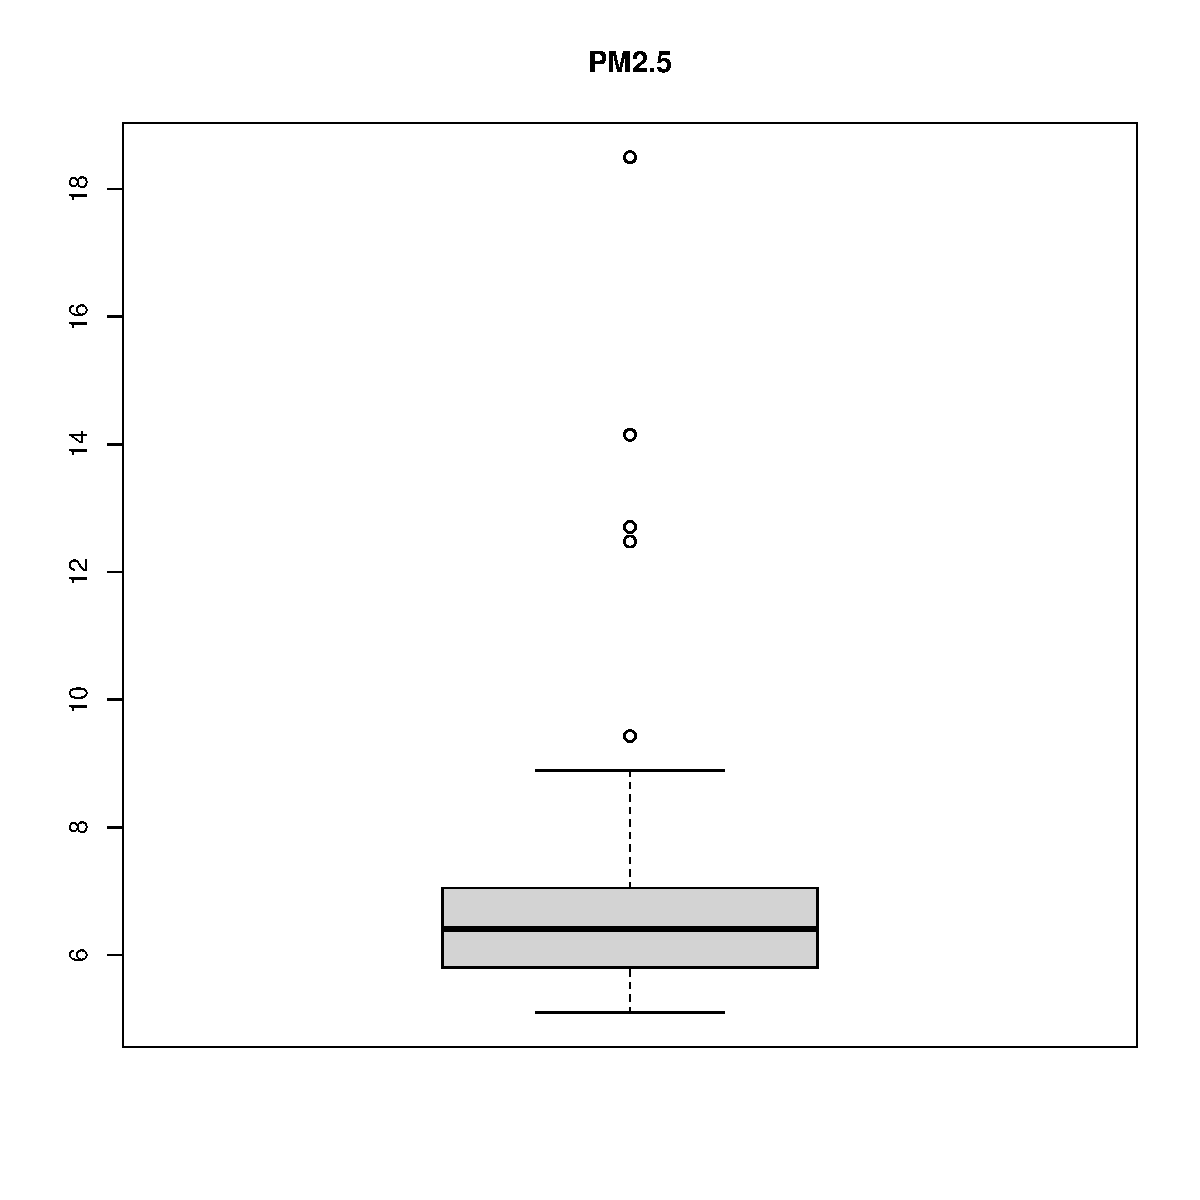
\includegraphics[width=0.4\linewidth]{figures/PM25_box.pdf}
    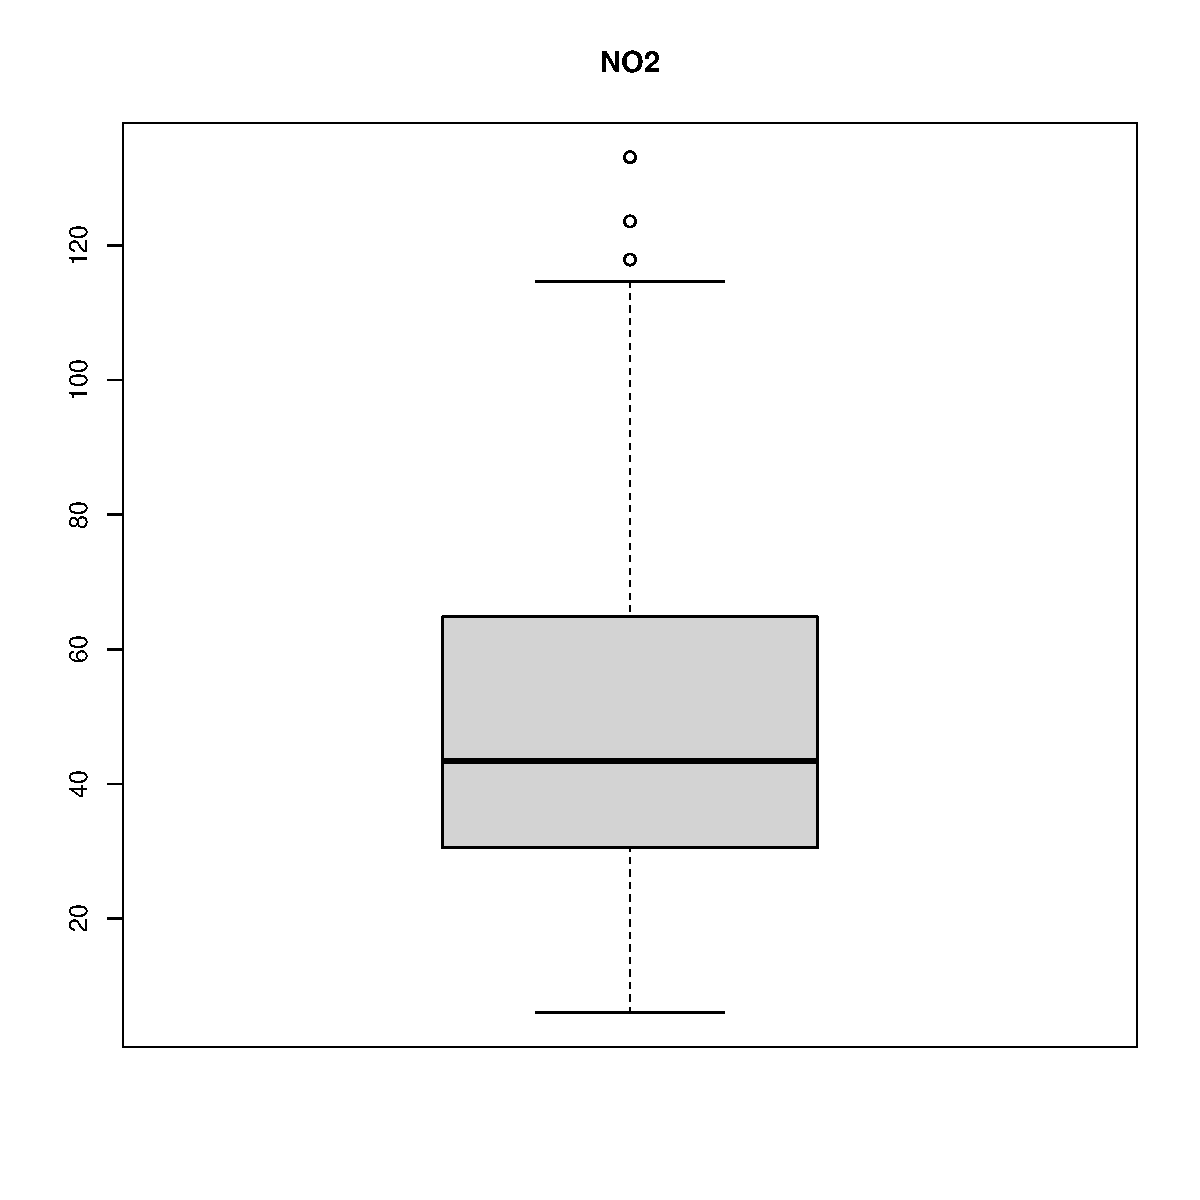
\includegraphics[width=0.4\linewidth]{figures/NO2_box.pdf}
    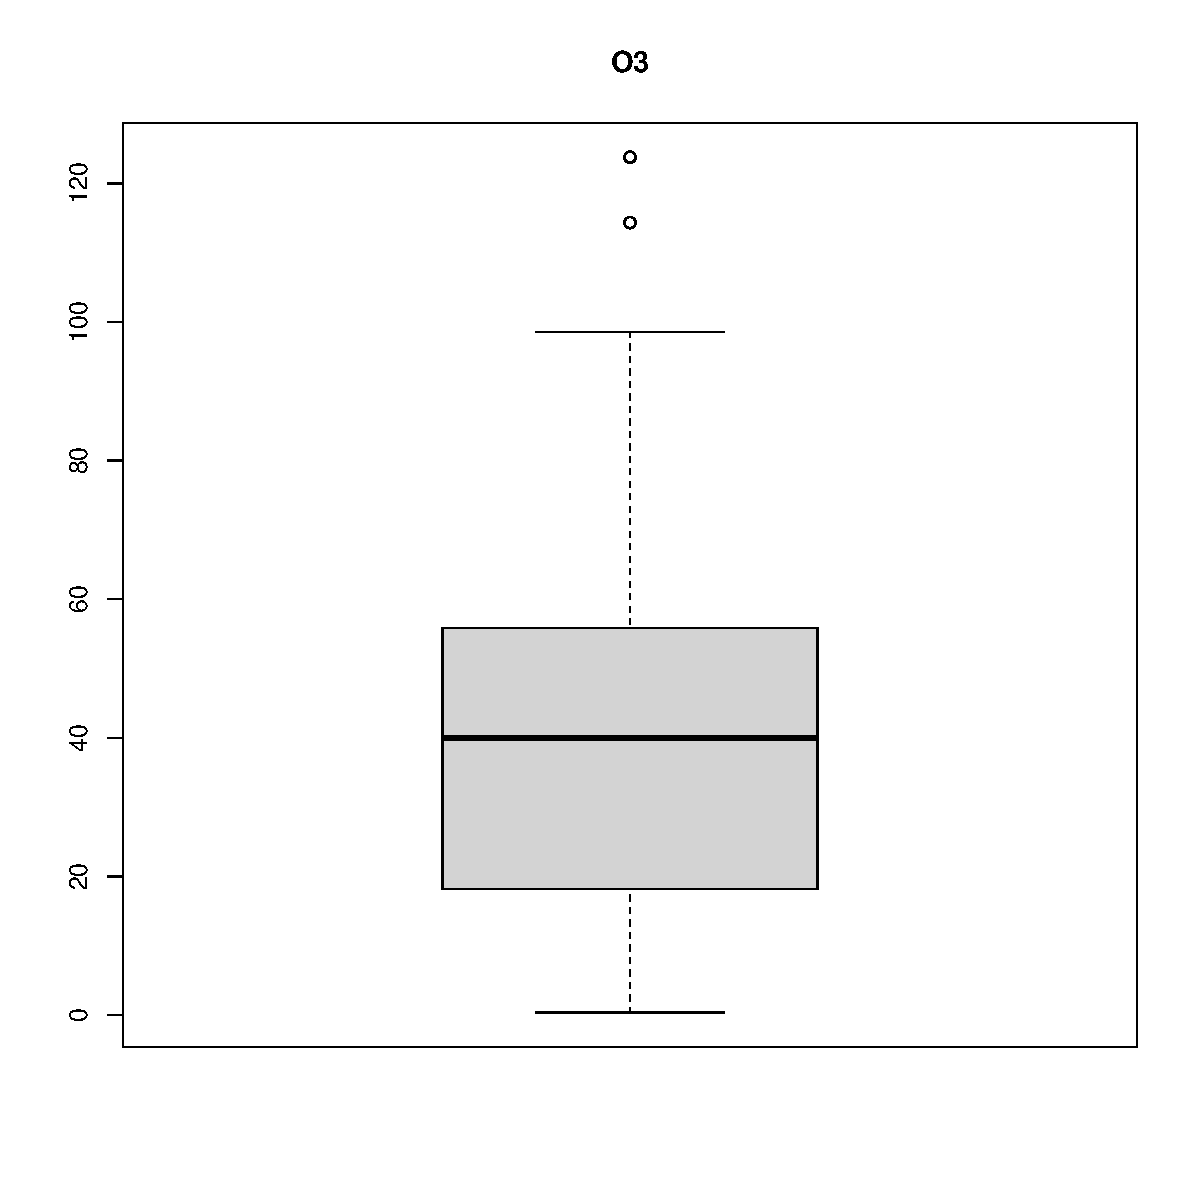
\includegraphics[width=0.4\linewidth]{figures/O3_box.pdf}
    \caption{PM2.5 box}
\end{figure}
% \subsection{NO2}
% \begin{figure}[H]
%     \centering
%     \vspace{-0.35cm}
%     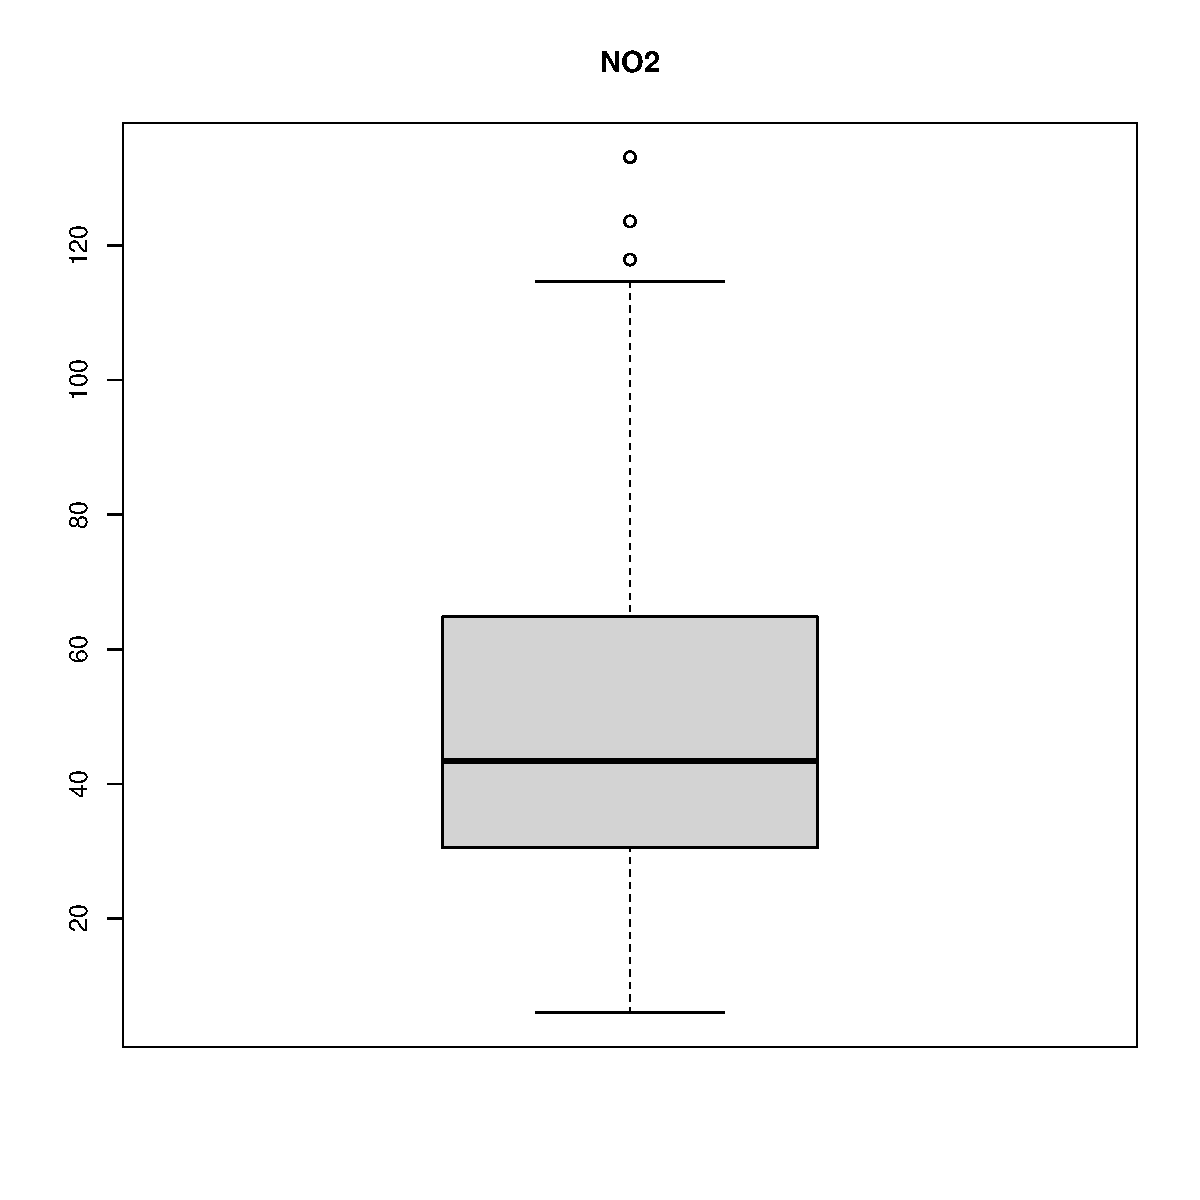
\includegraphics[width=0.7\linewidth]{figures/NO2_box.pdf}
%     \caption{NO2 box}
% \end{figure}
% \subsection{O3}
% \begin{figure}[H]
%     \centering
%     \vspace{-0.35cm}
%     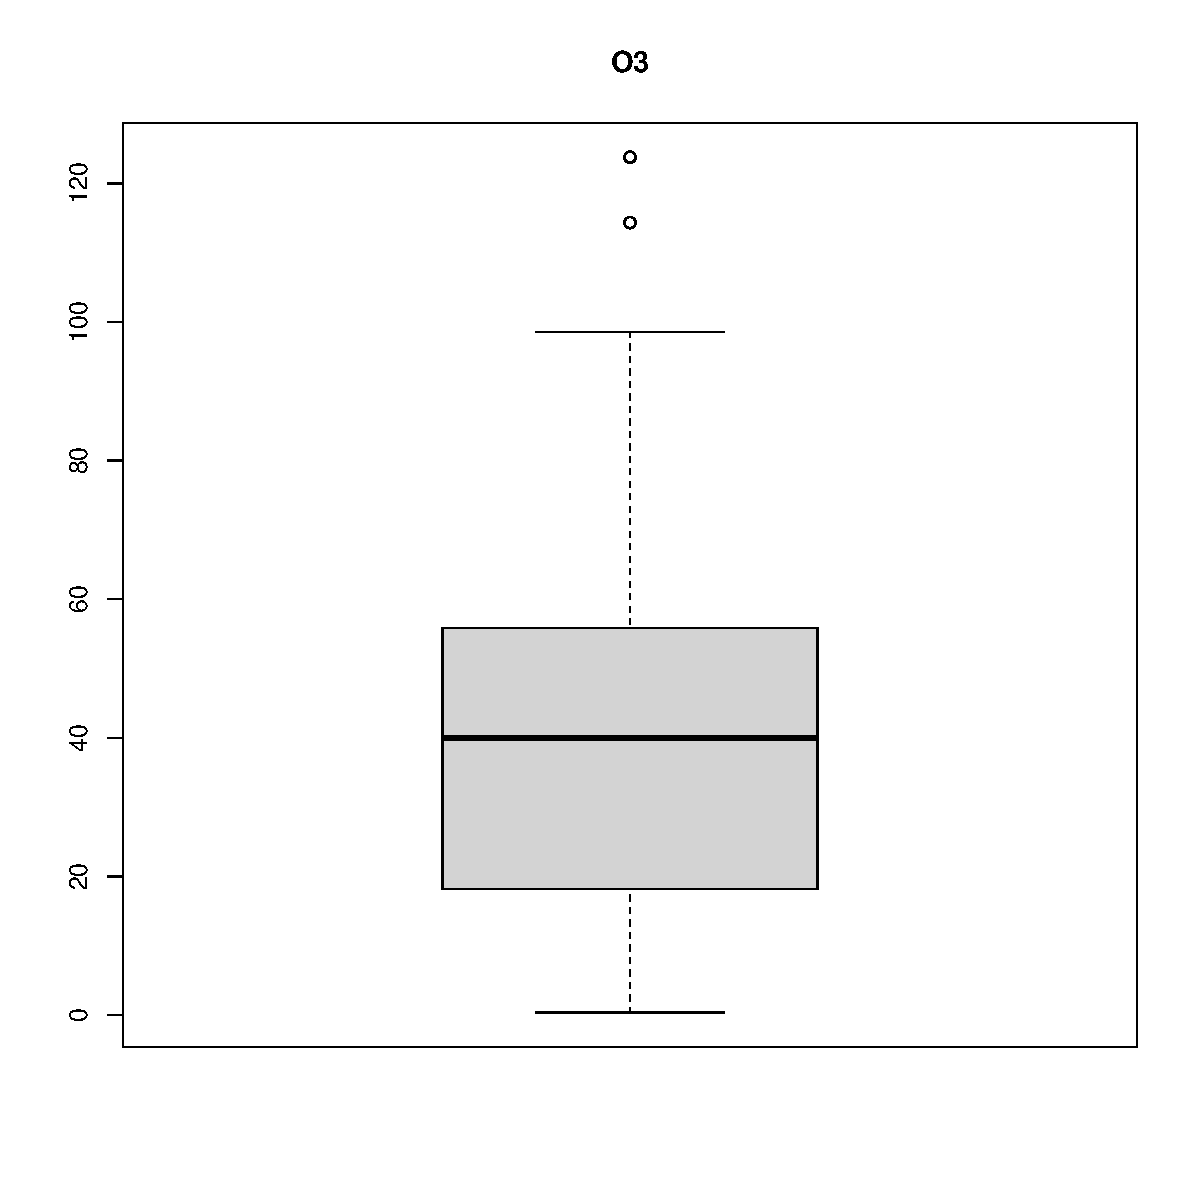
\includegraphics[width=0.7\linewidth]{figures/O3_box.pdf}
%     \caption{O3 box}
% \end{figure}

% --------------------------------------------------------
% Section 3: more advanced statistics
% --------------------------------------------------------
\section{more advanced statistics}
\label{sec:more advanced statistics}
\subsection{PM2.5}
% \begin{figure}[H]
%     \centering
%     \vspace{-0.35cm}
%     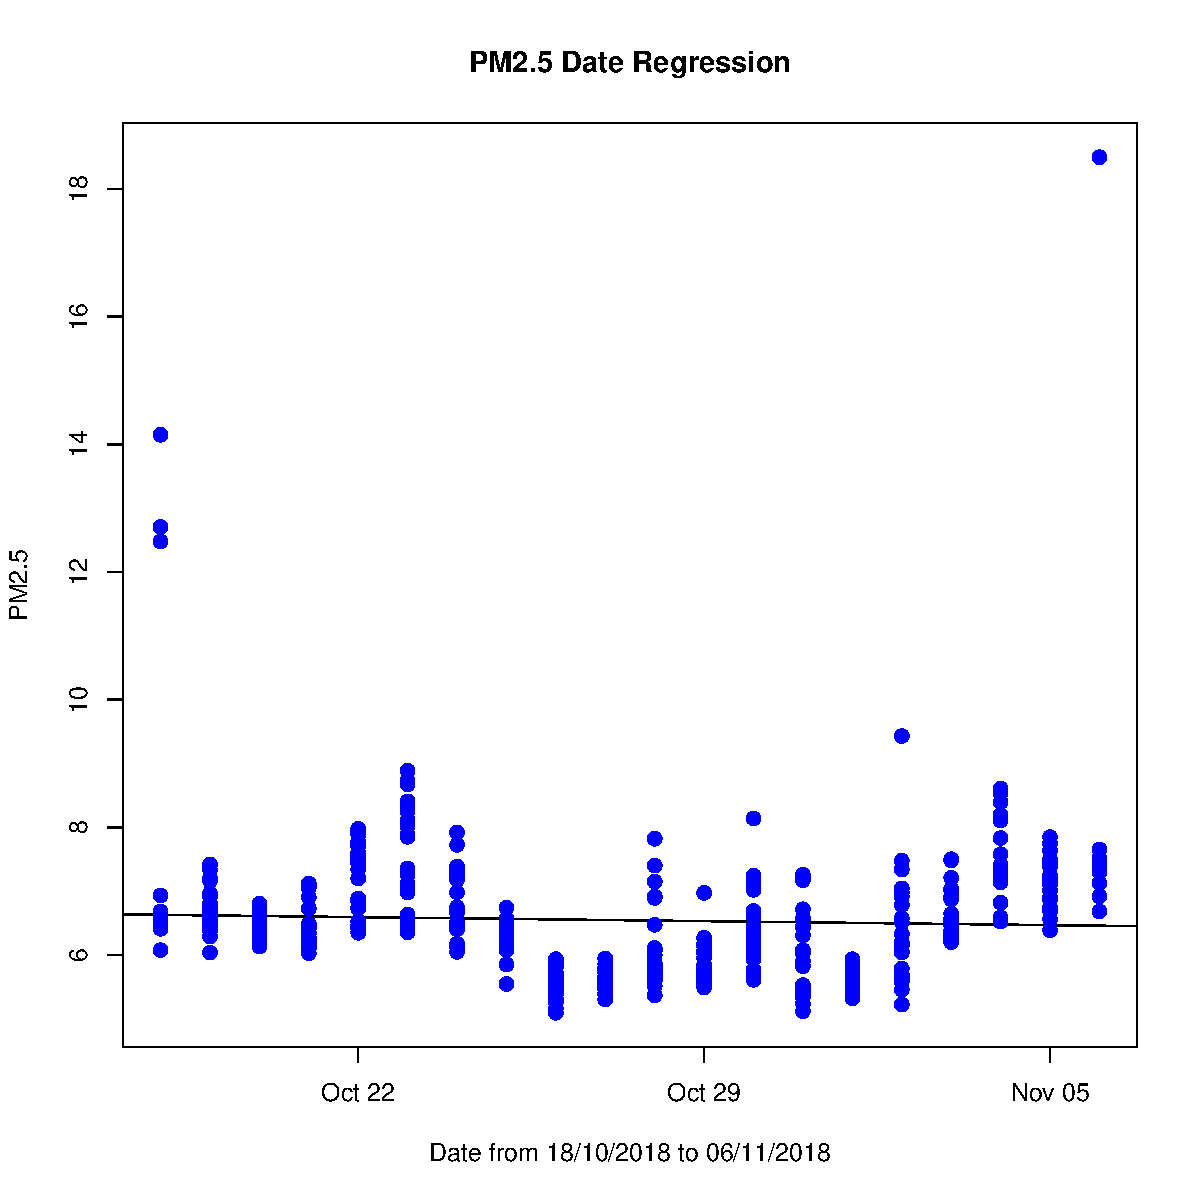
\includegraphics[width=0.7\linewidth]{figures/PM25_Date_Regression.pdf}
%     % \caption{}
% \end{figure}
% \begin{figure}[H]
%     \centering
%     \vspace{-0.35cm}
%     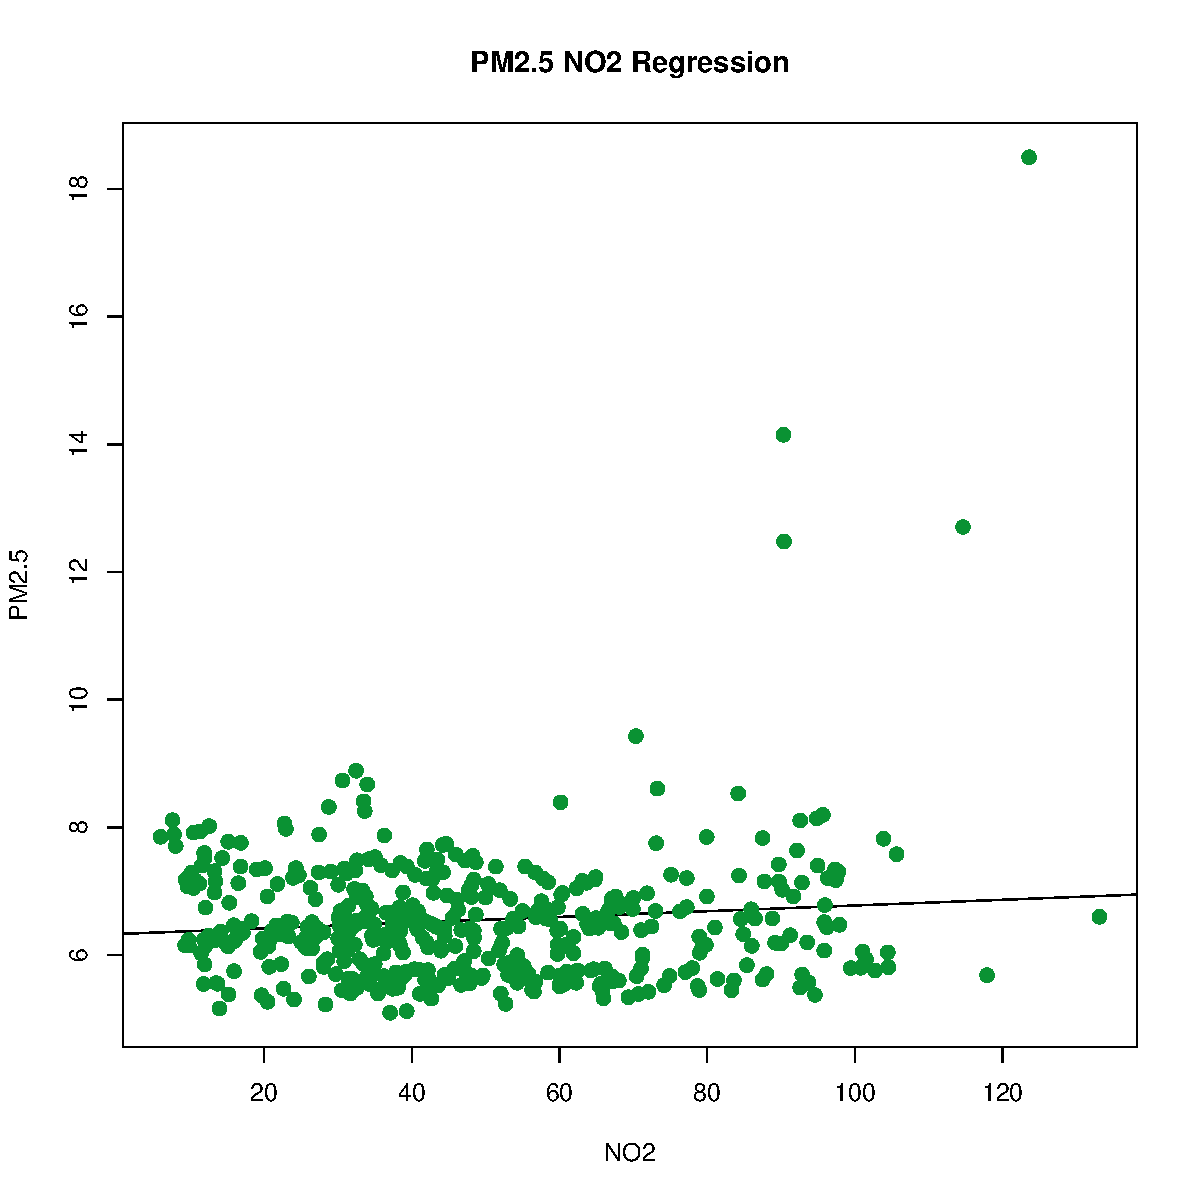
\includegraphics[width=0.7\linewidth]{figures/PM25_NO2_Regression.pdf}
%     % \caption{}
% \end{figure}
% \begin{figure}[H]
%     \centering
%     \vspace{-0.35cm}
%     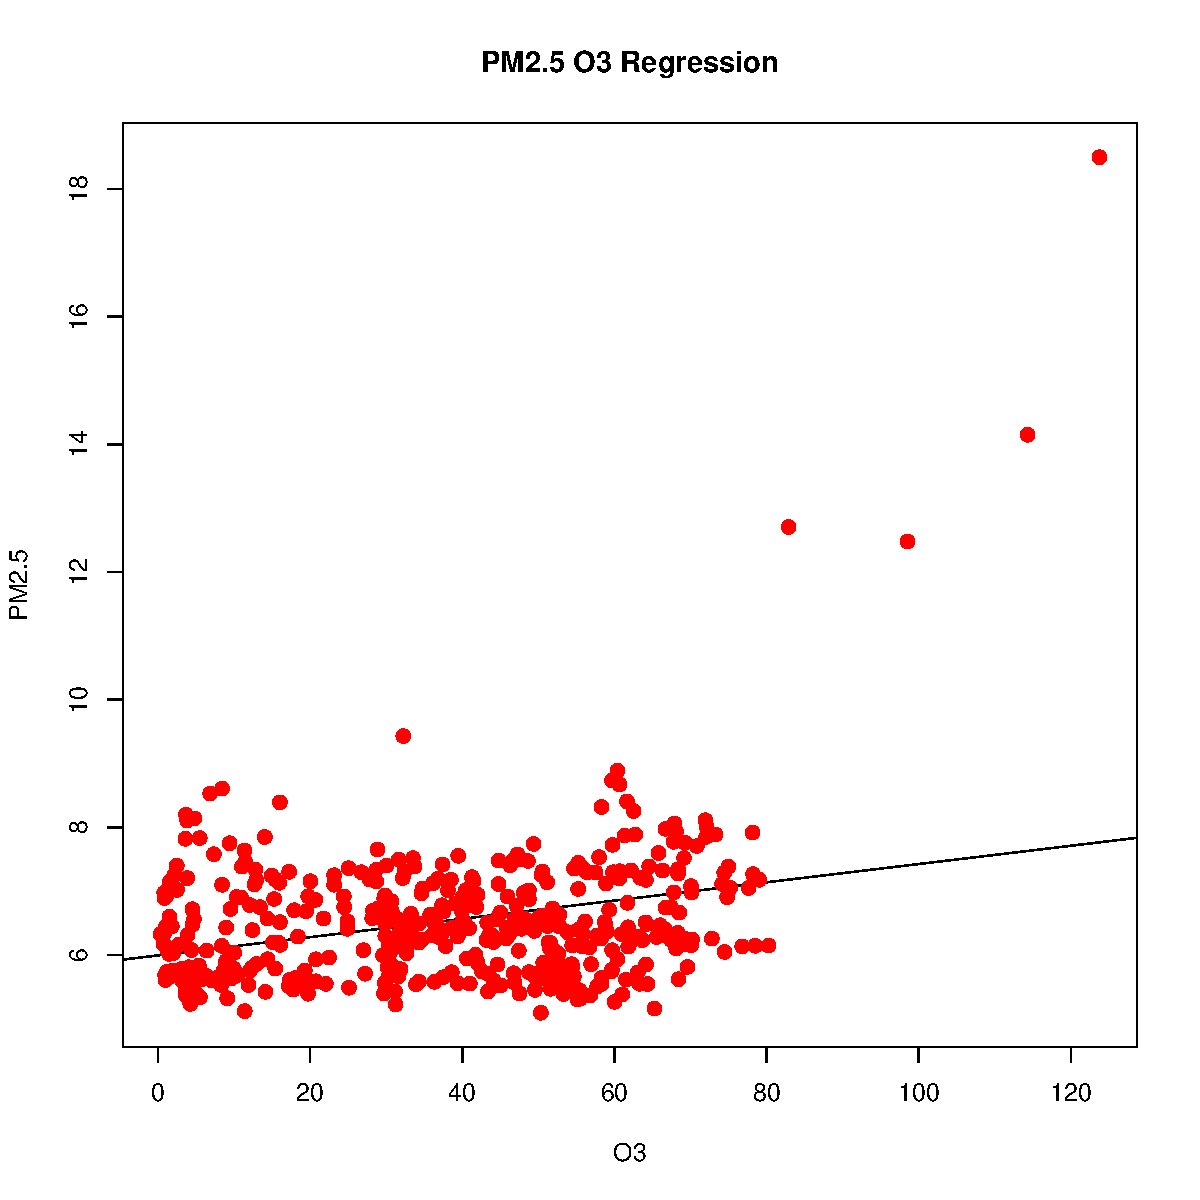
\includegraphics[width=0.7\linewidth]{figures/PM25_O3_Regression.pdf}
%     % \caption{}
% \end{figure}
% \begin{figure}[H]
%     \centering
%     \vspace{-0.35cm}
%     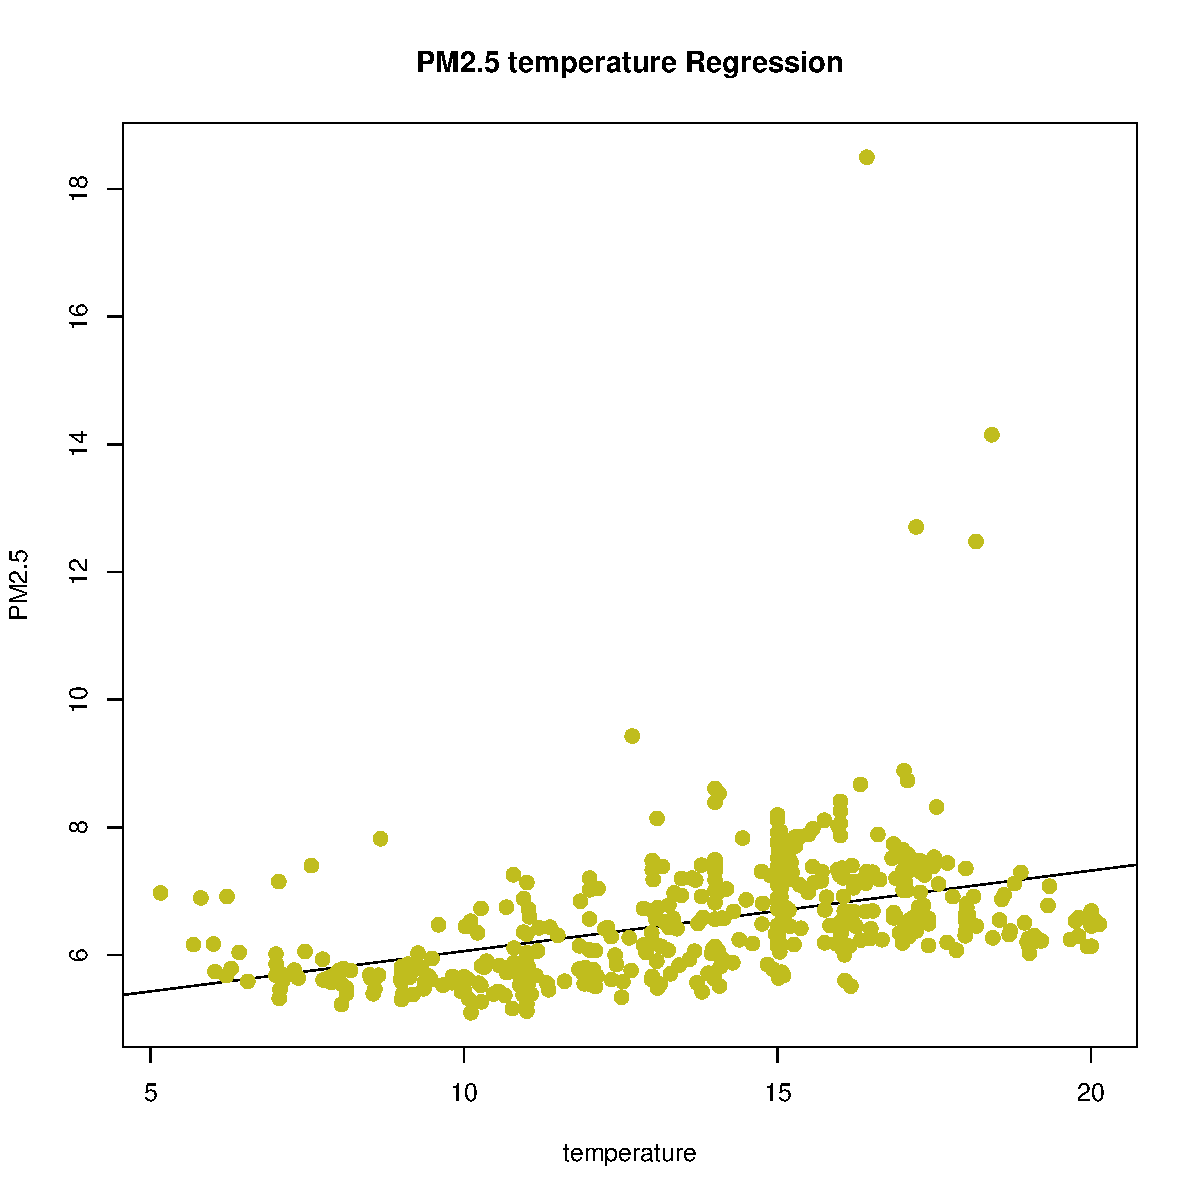
\includegraphics[width=0.7\linewidth]{figures/PM25_temperature_Regression.pdf}
%     % \caption{}
% \end{figure}
% \begin{figure}[H]
%     \centering
%     \vspace{-0.35cm}
%     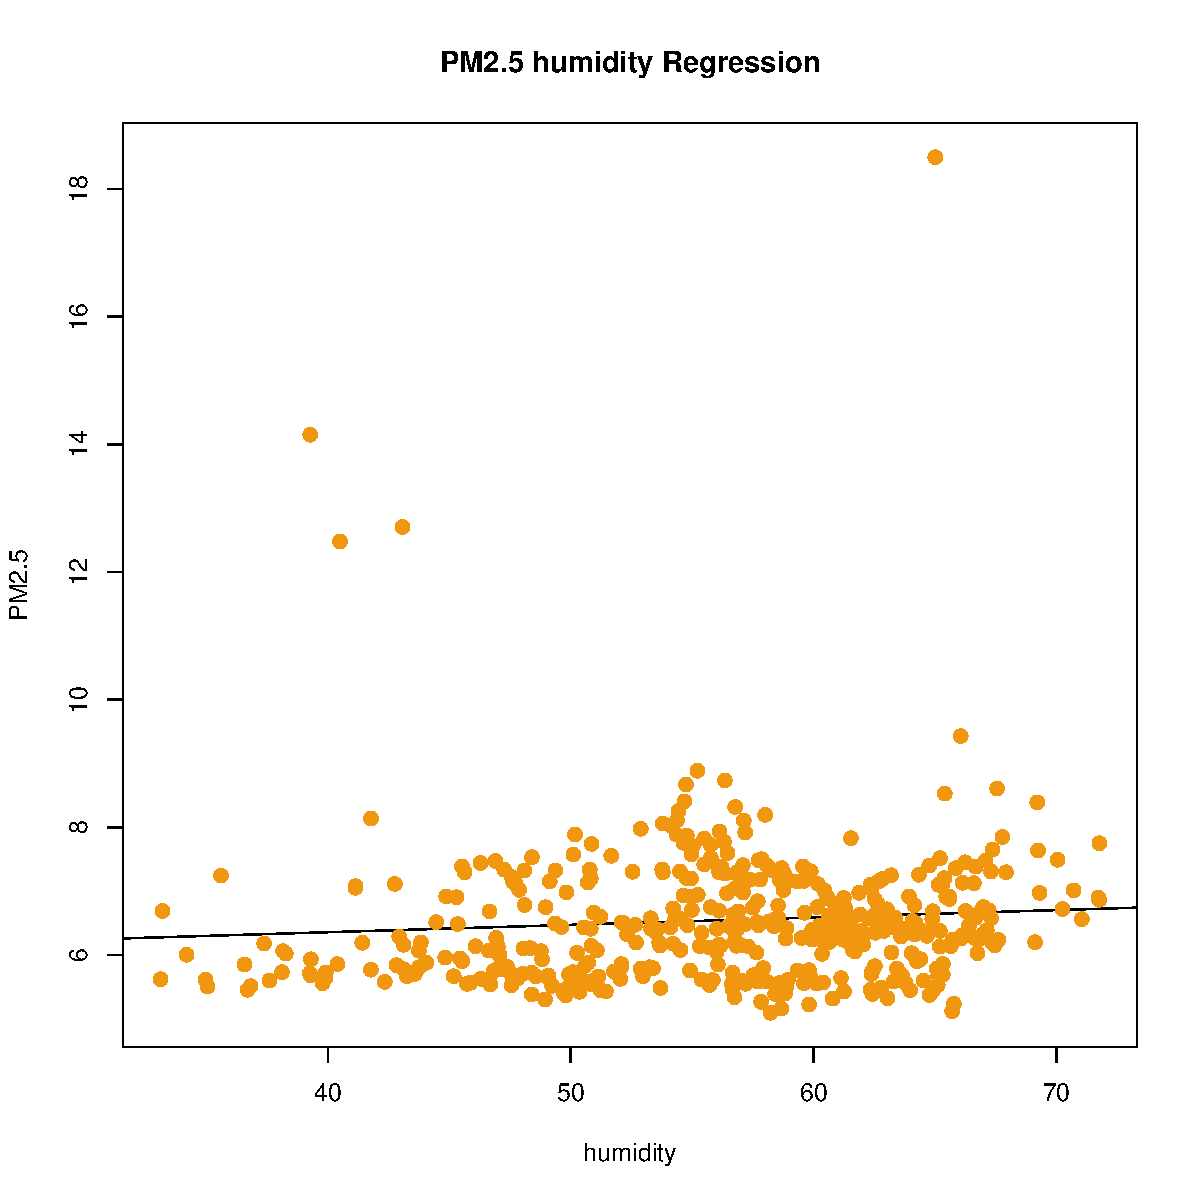
\includegraphics[width=0.7\linewidth]{figures/PM25_humidity_Regression.pdf}
%     % \caption{}
% \end{figure}
\begin{figure}[H]
    \centering
    \vspace{-0.35cm}
    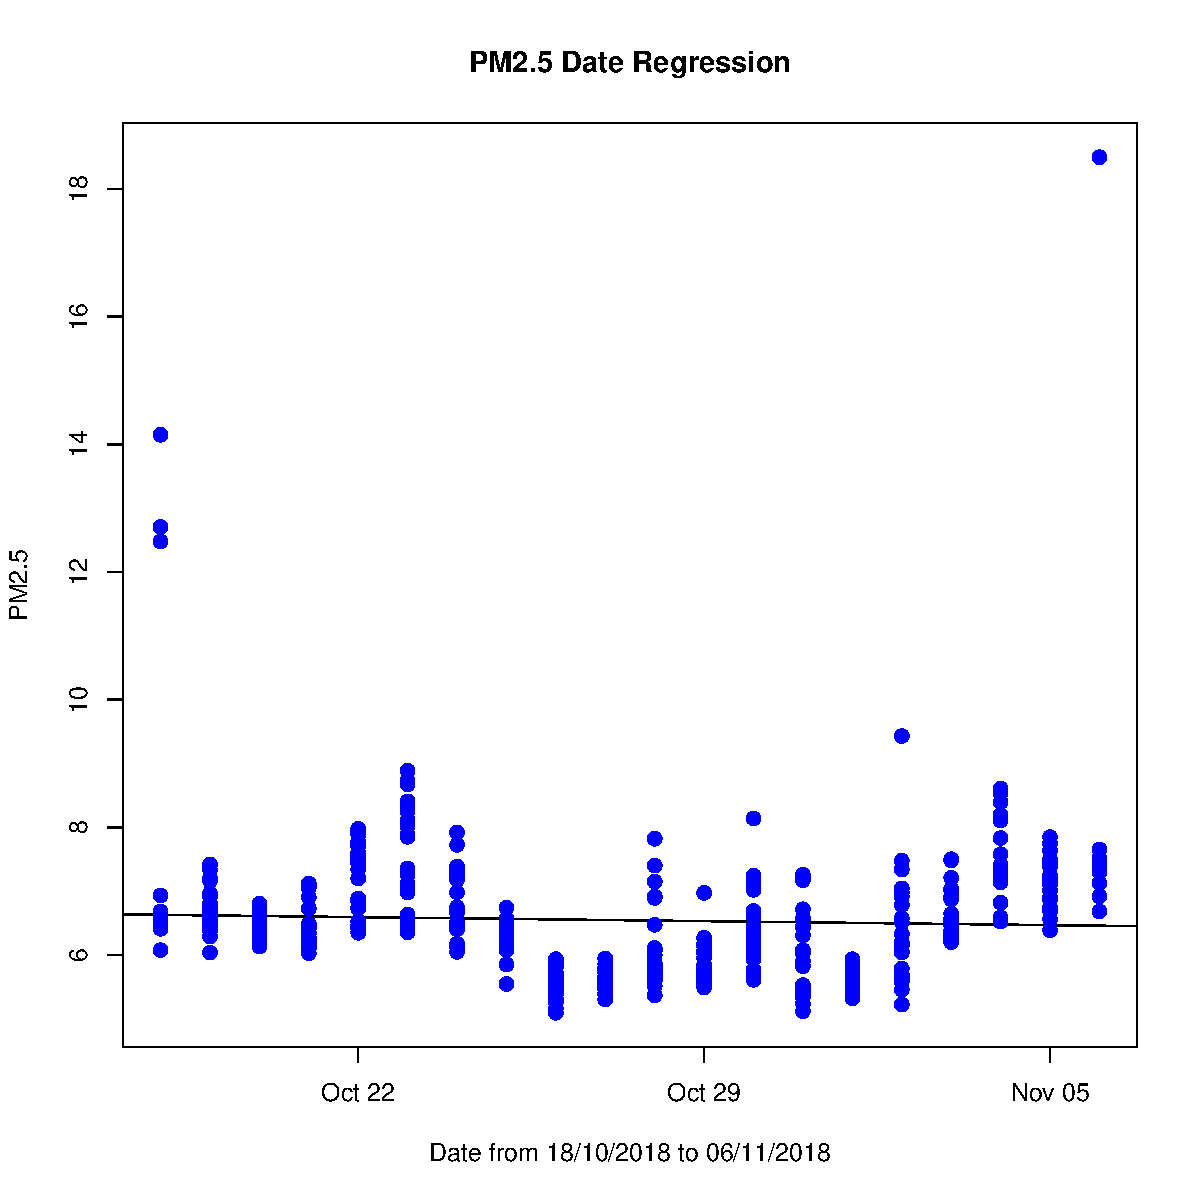
\includegraphics[width=0.4\linewidth]{figures/PM25_Date_Regression.pdf}
    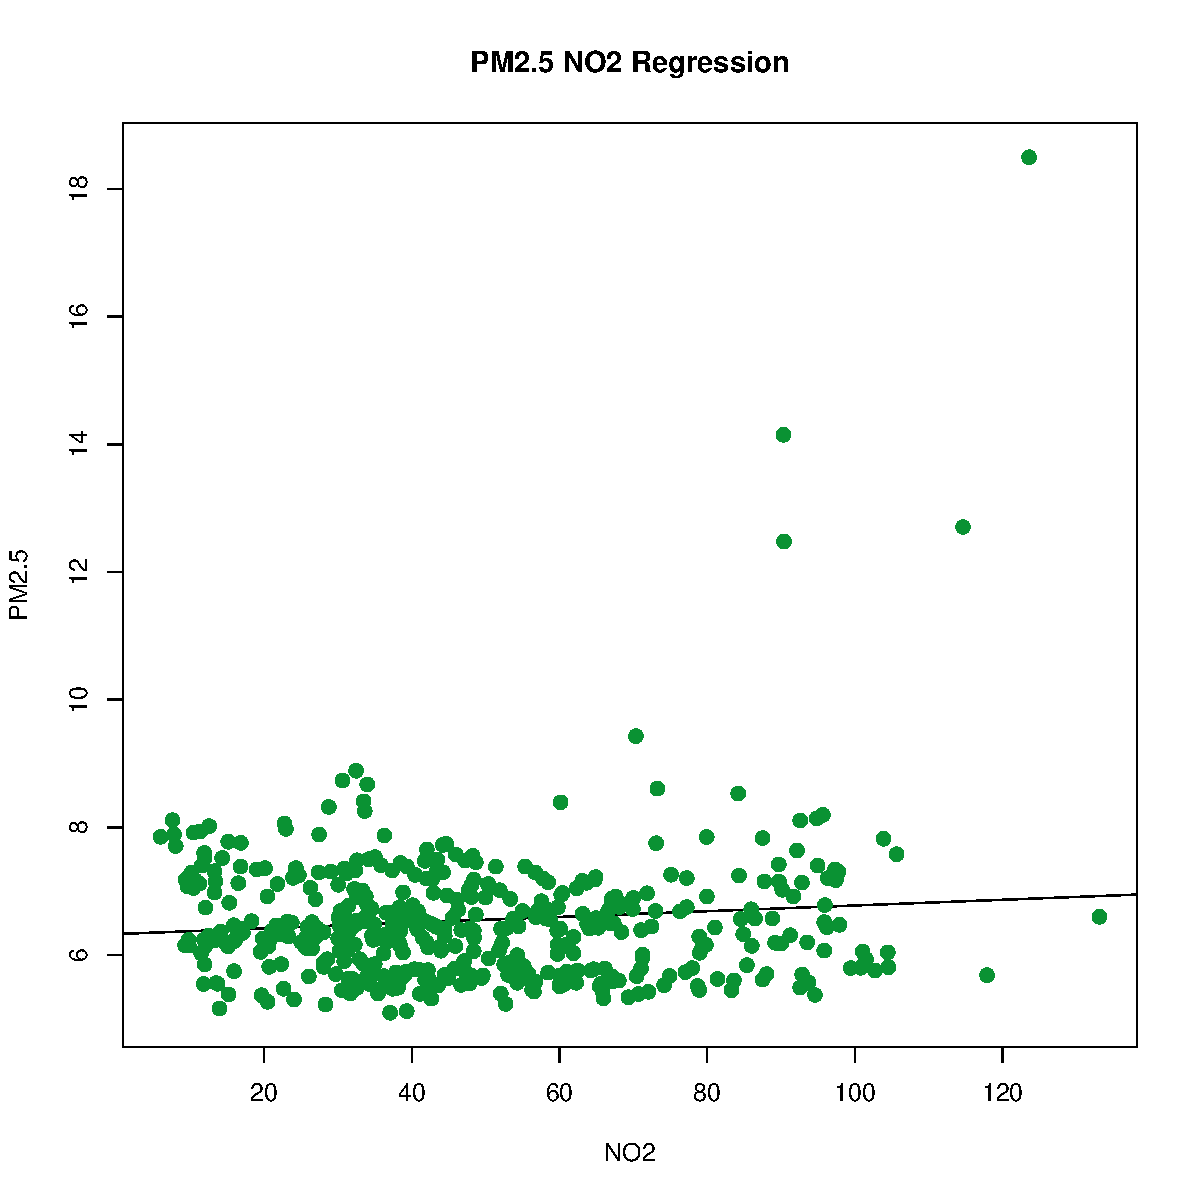
\includegraphics[width=0.4\linewidth]{figures/PM25_NO2_Regression.pdf}
    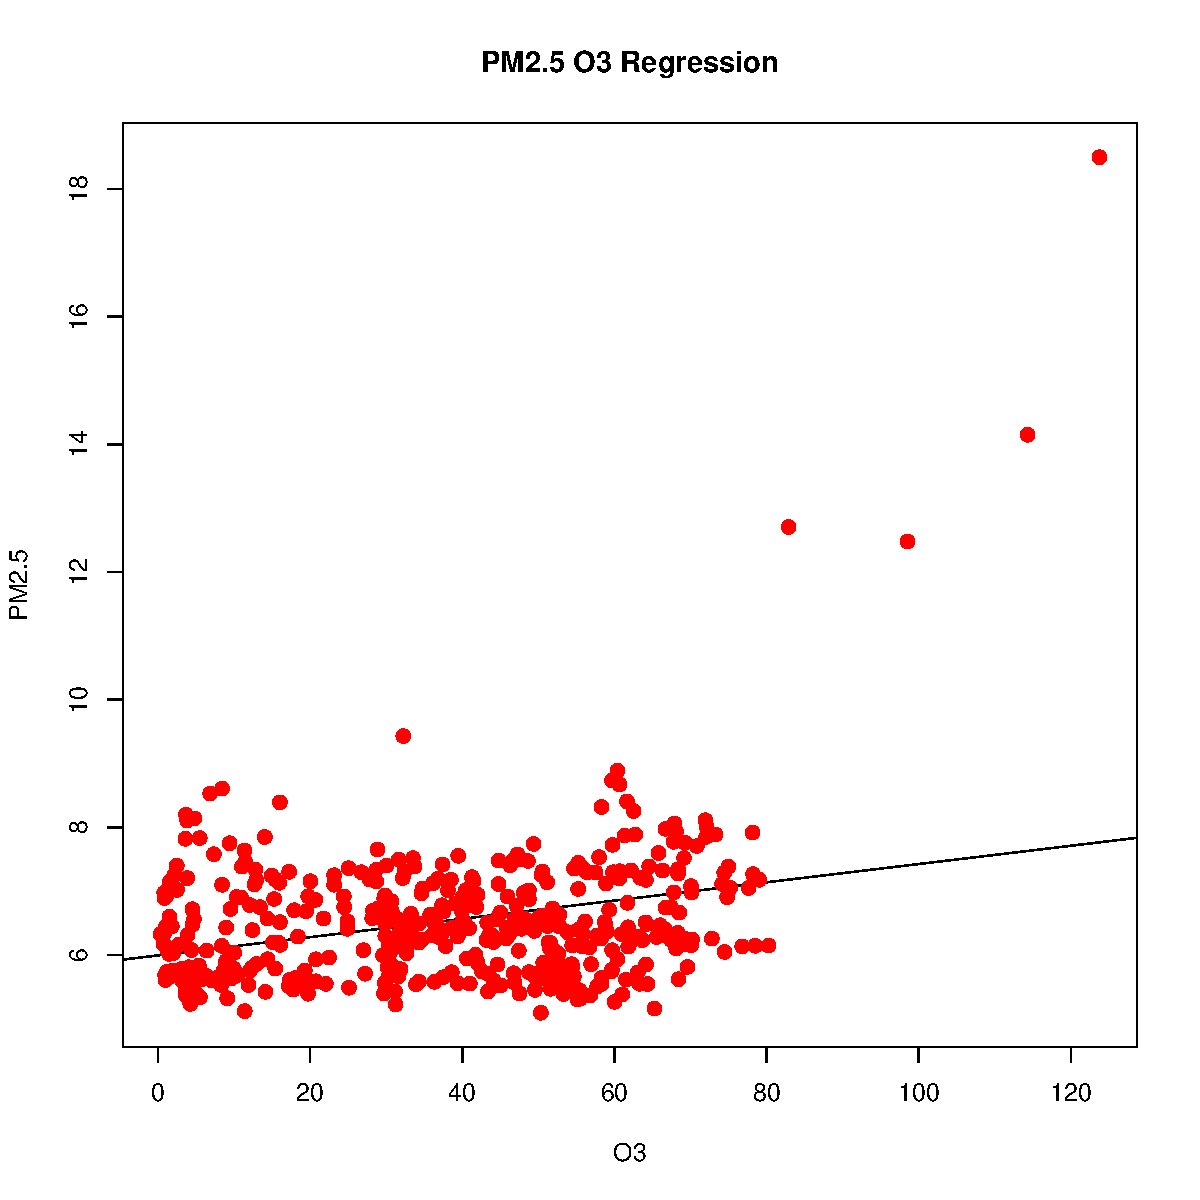
\includegraphics[width=0.4\linewidth]{figures/PM25_O3_Regression.pdf}
    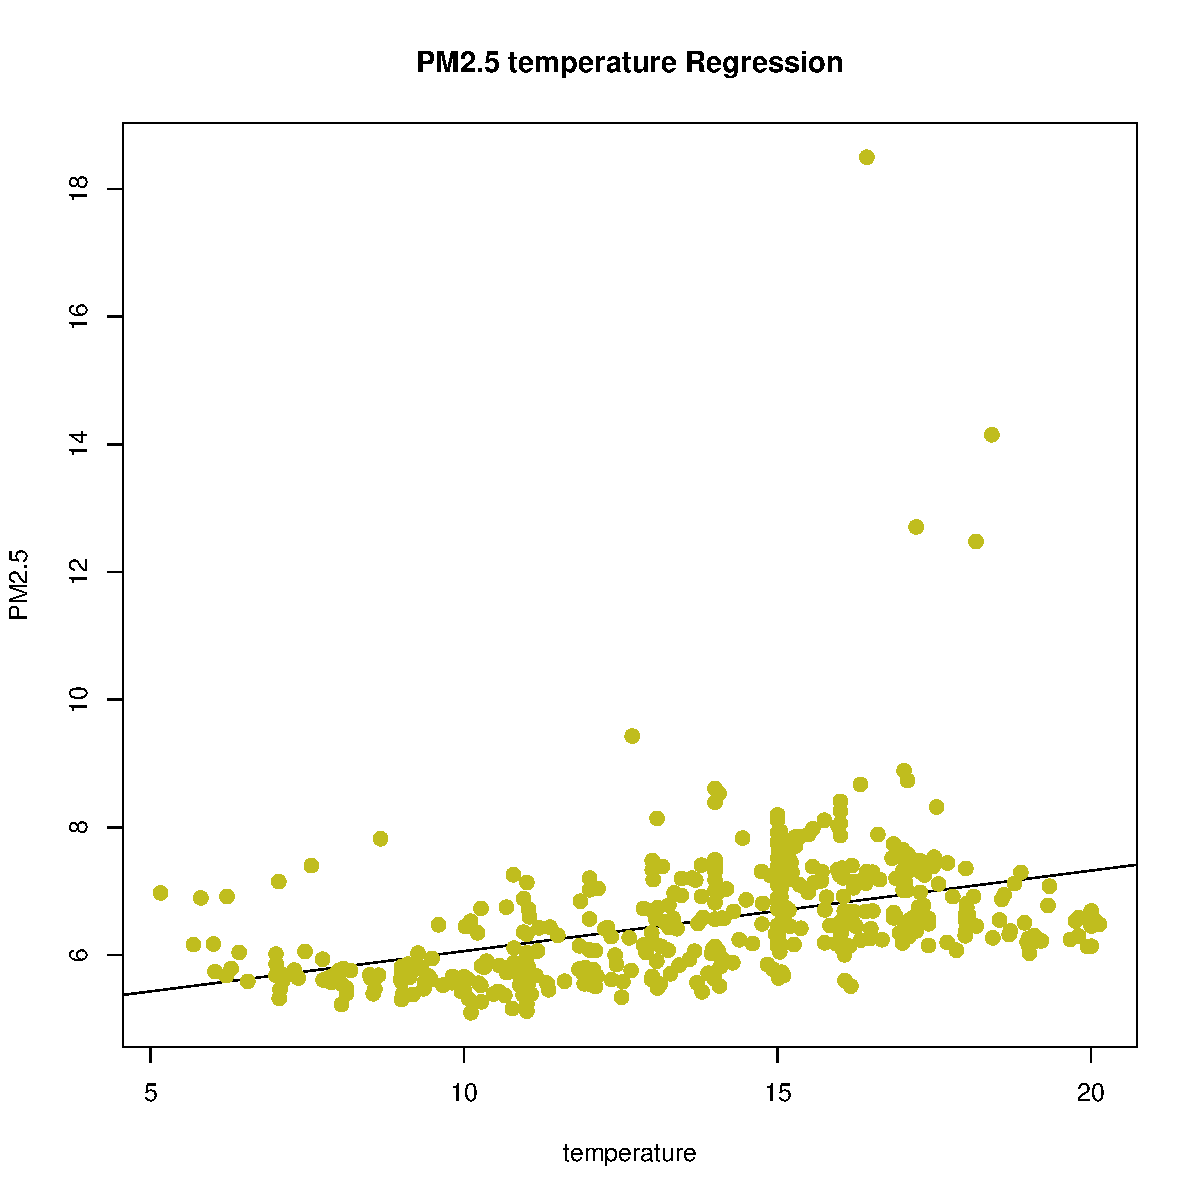
\includegraphics[width=0.4\linewidth]{figures/PM25_temperature_Regression.pdf}
    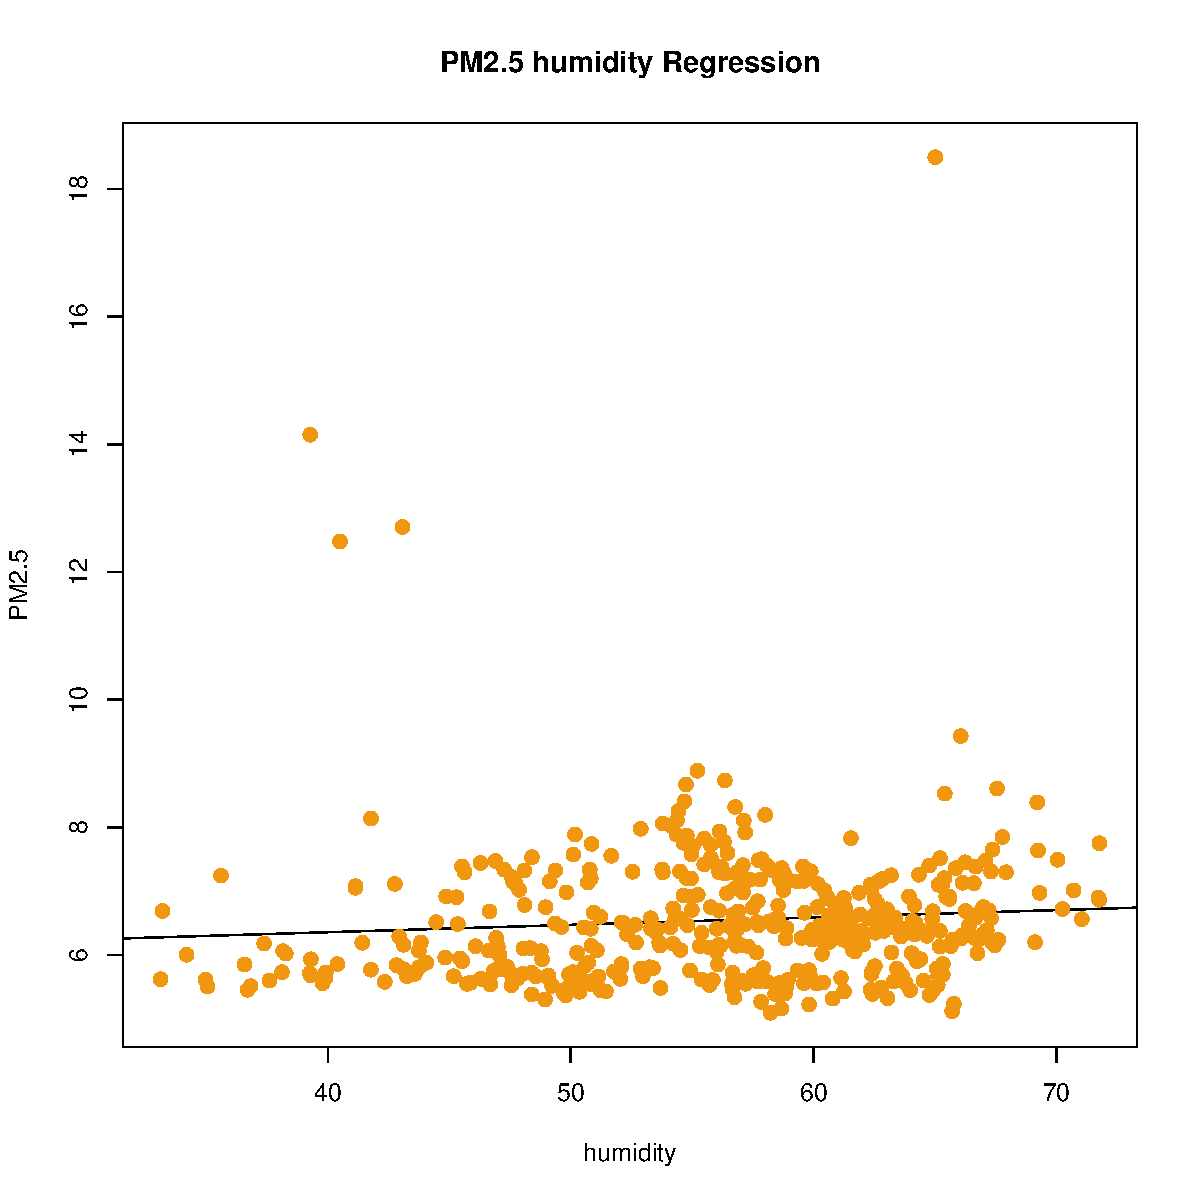
\includegraphics[width=0.4\linewidth]{figures/PM25_humidity_Regression.pdf}
    % \caption{}
\end{figure}
\subsection{NO2}
\begin{figure}[H]
    \centering
    \vspace{-0.35cm}
    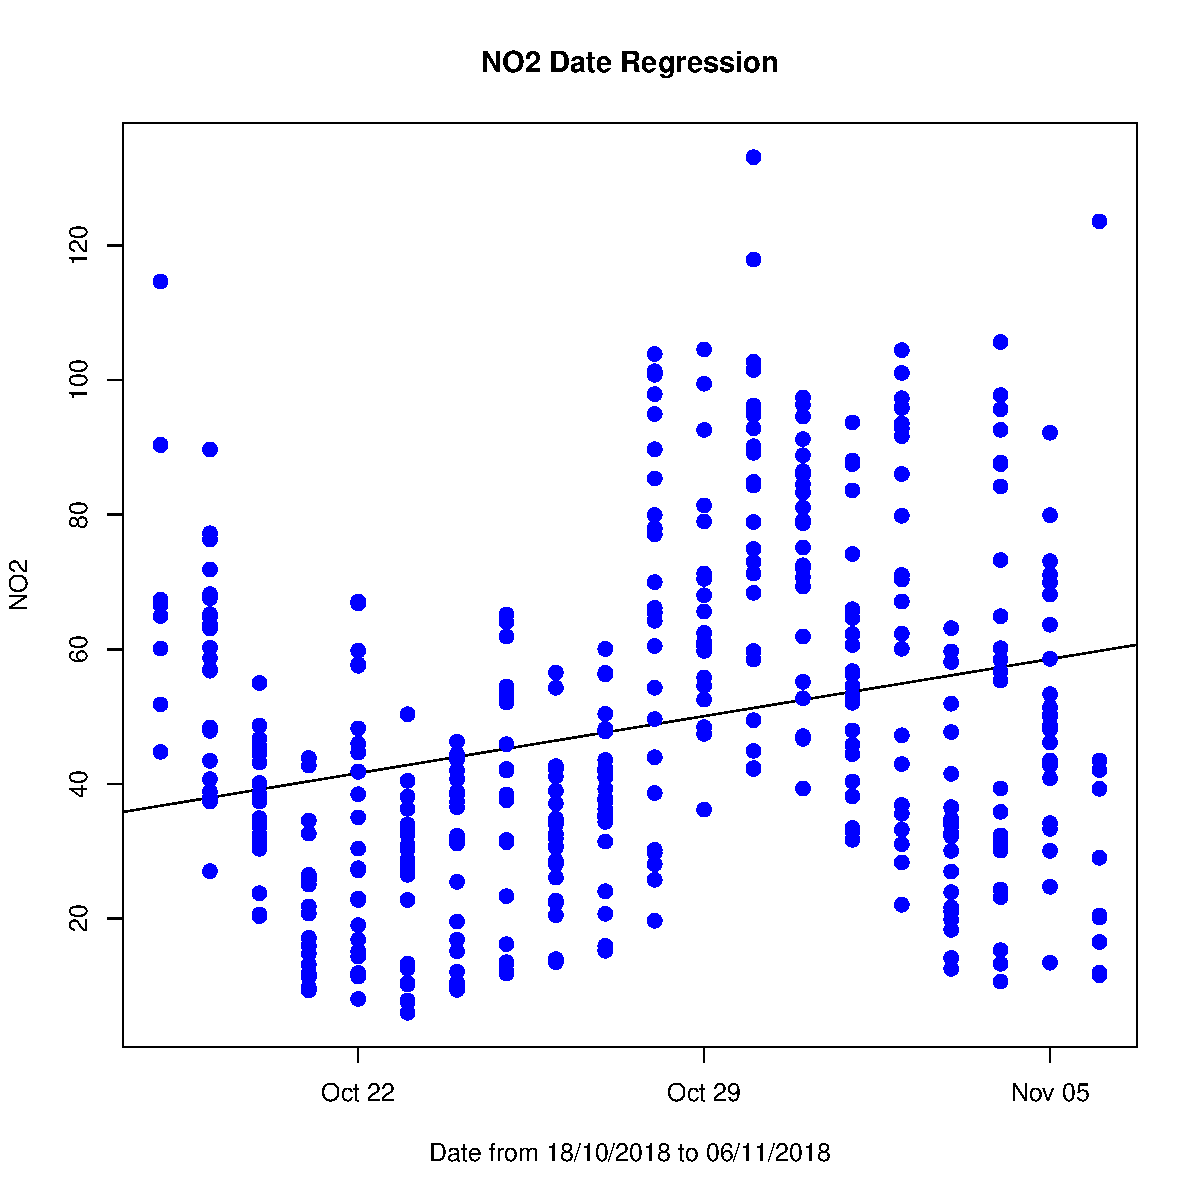
\includegraphics[width=0.4\linewidth]{figures/NO2_Date_Regression.pdf}
    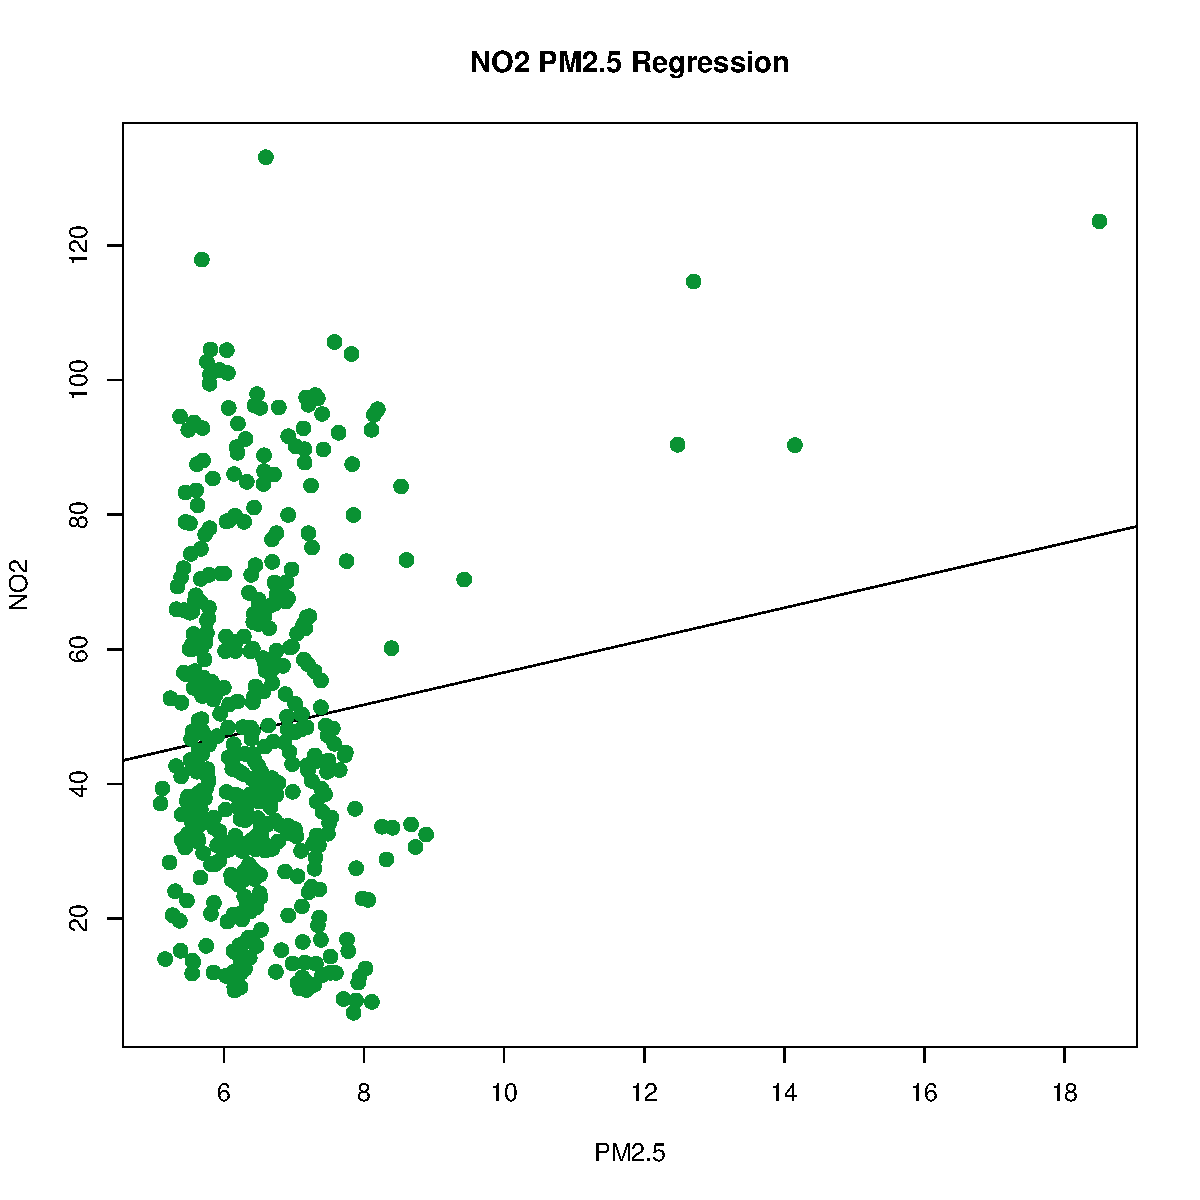
\includegraphics[width=0.4\linewidth]{figures/NO2_PM25_Regression.pdf}
    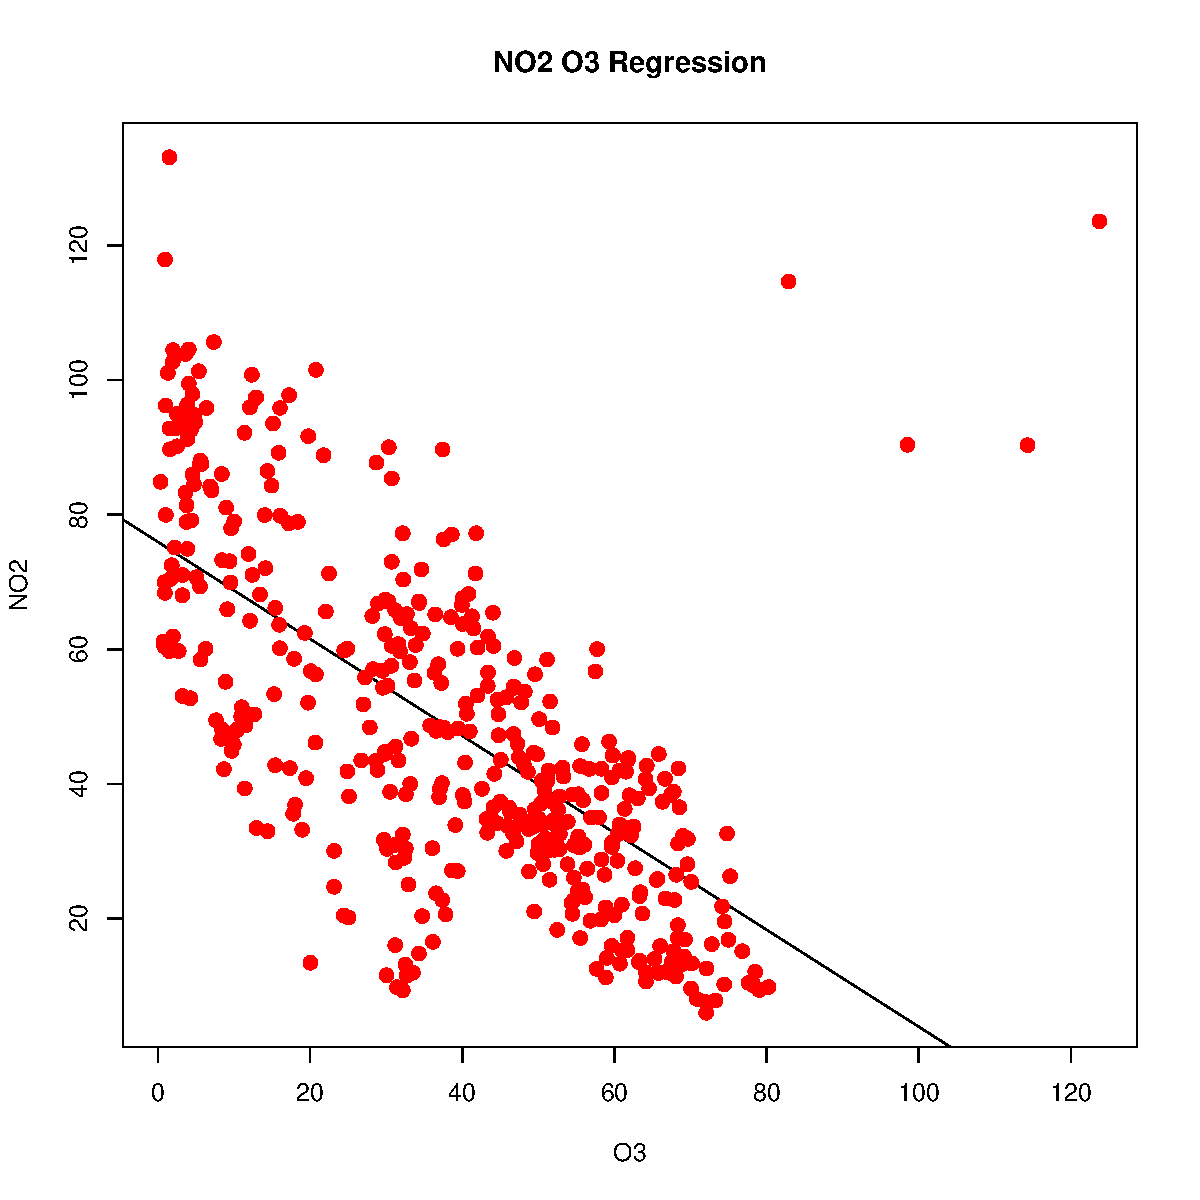
\includegraphics[width=0.4\linewidth]{figures/NO2_O3_Regression.pdf}
    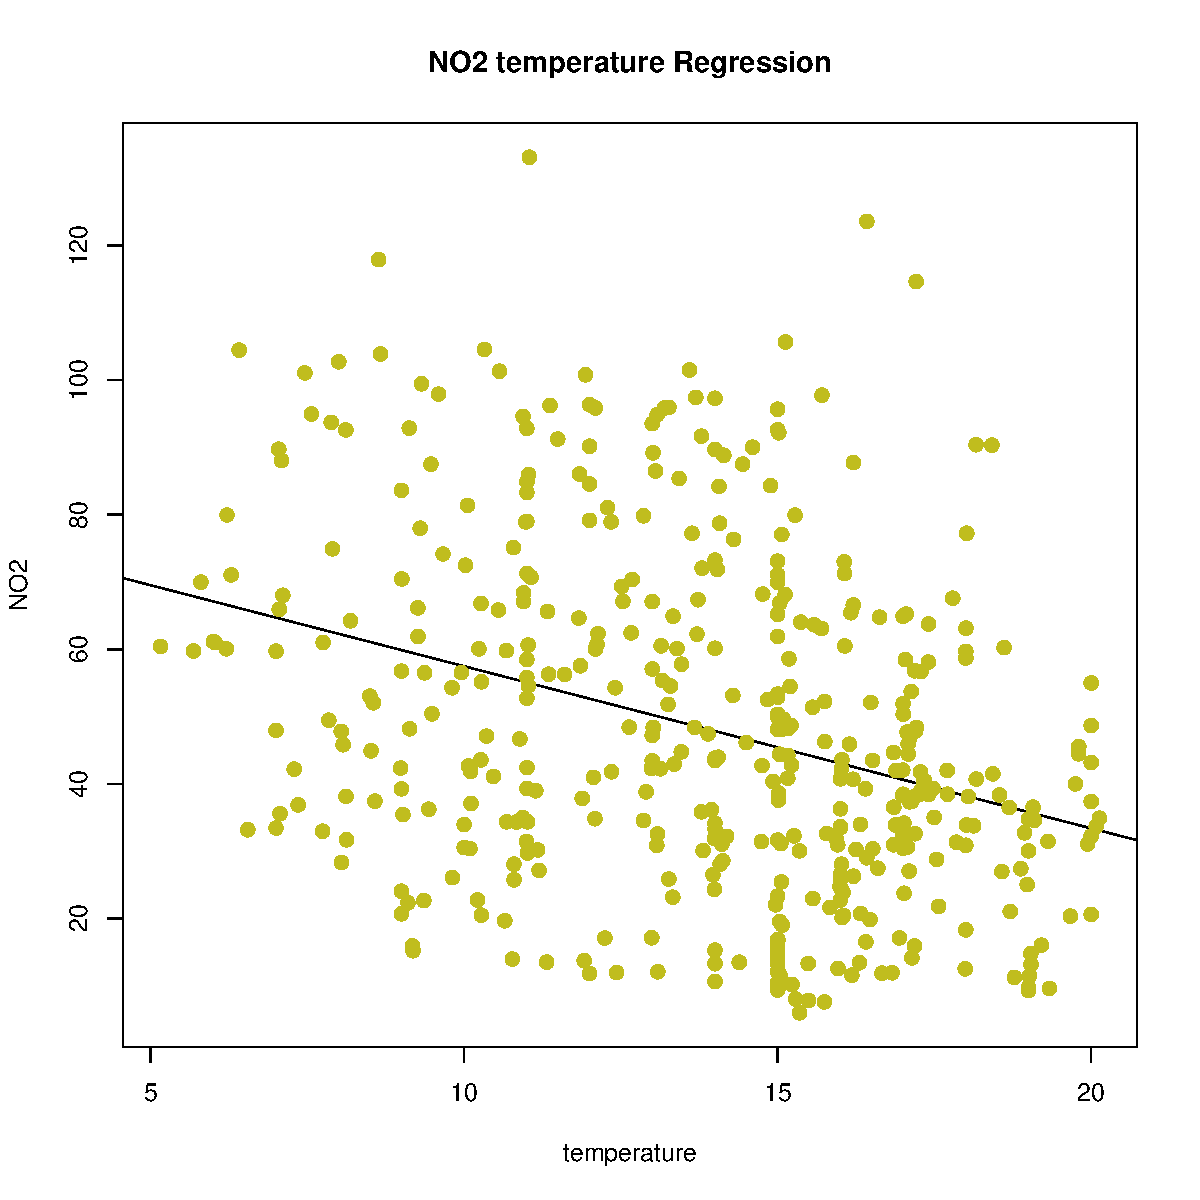
\includegraphics[width=0.4\linewidth]{figures/NO2_temperature_Regression.pdf}
    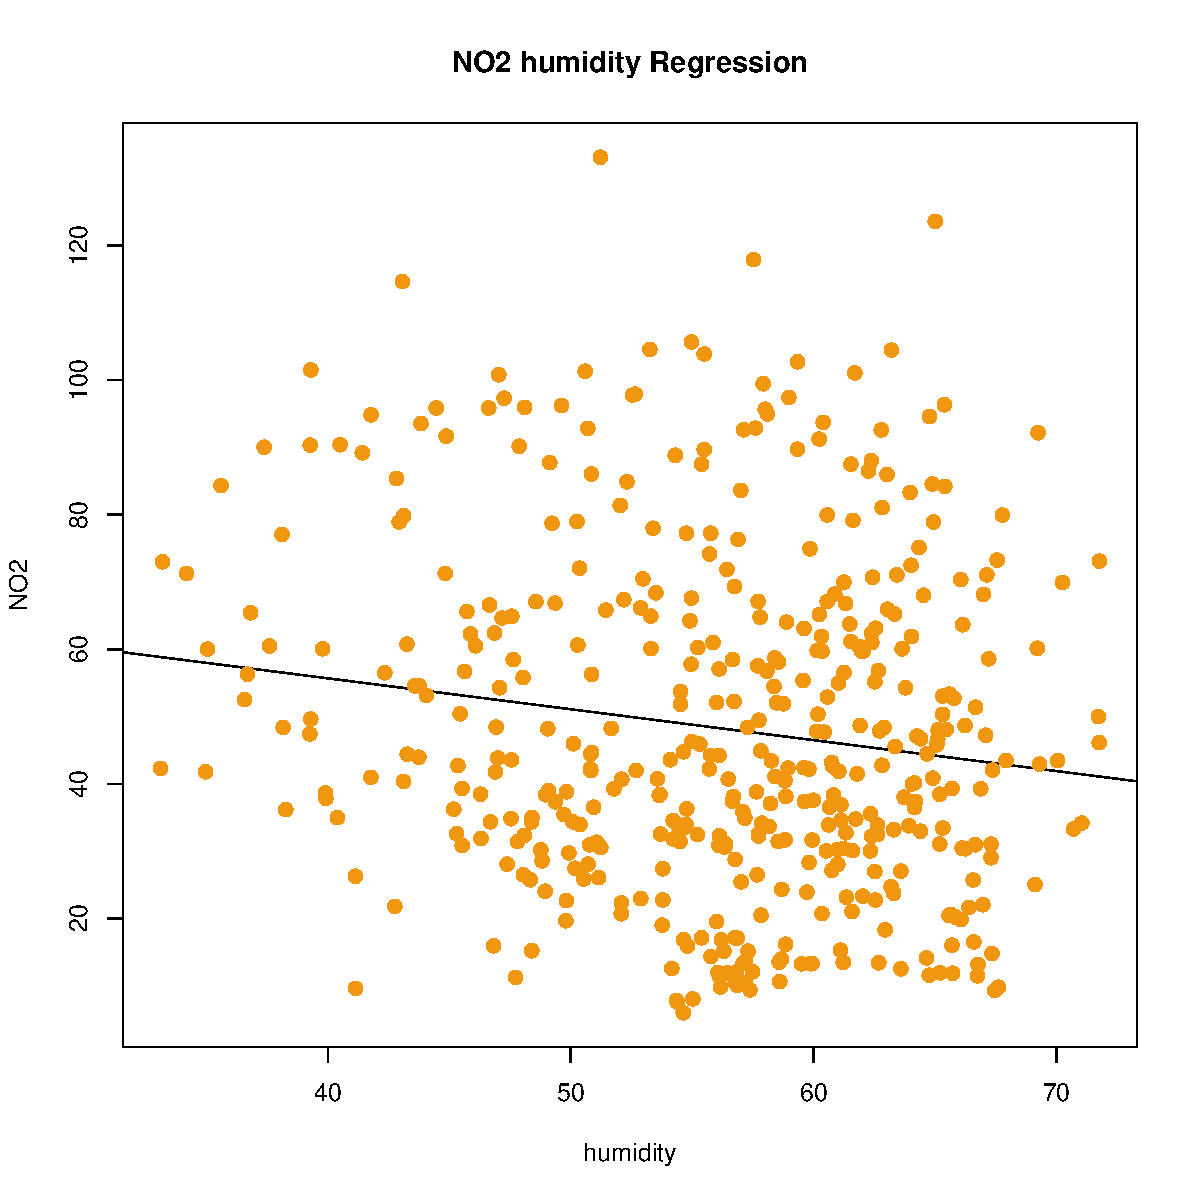
\includegraphics[width=0.4\linewidth]{figures/NO2_humidity_Regression.pdf}
    % \caption{}
\end{figure}
\subsection{O3}
\begin{figure}[H]
    \centering
    \vspace{-0.35cm}
    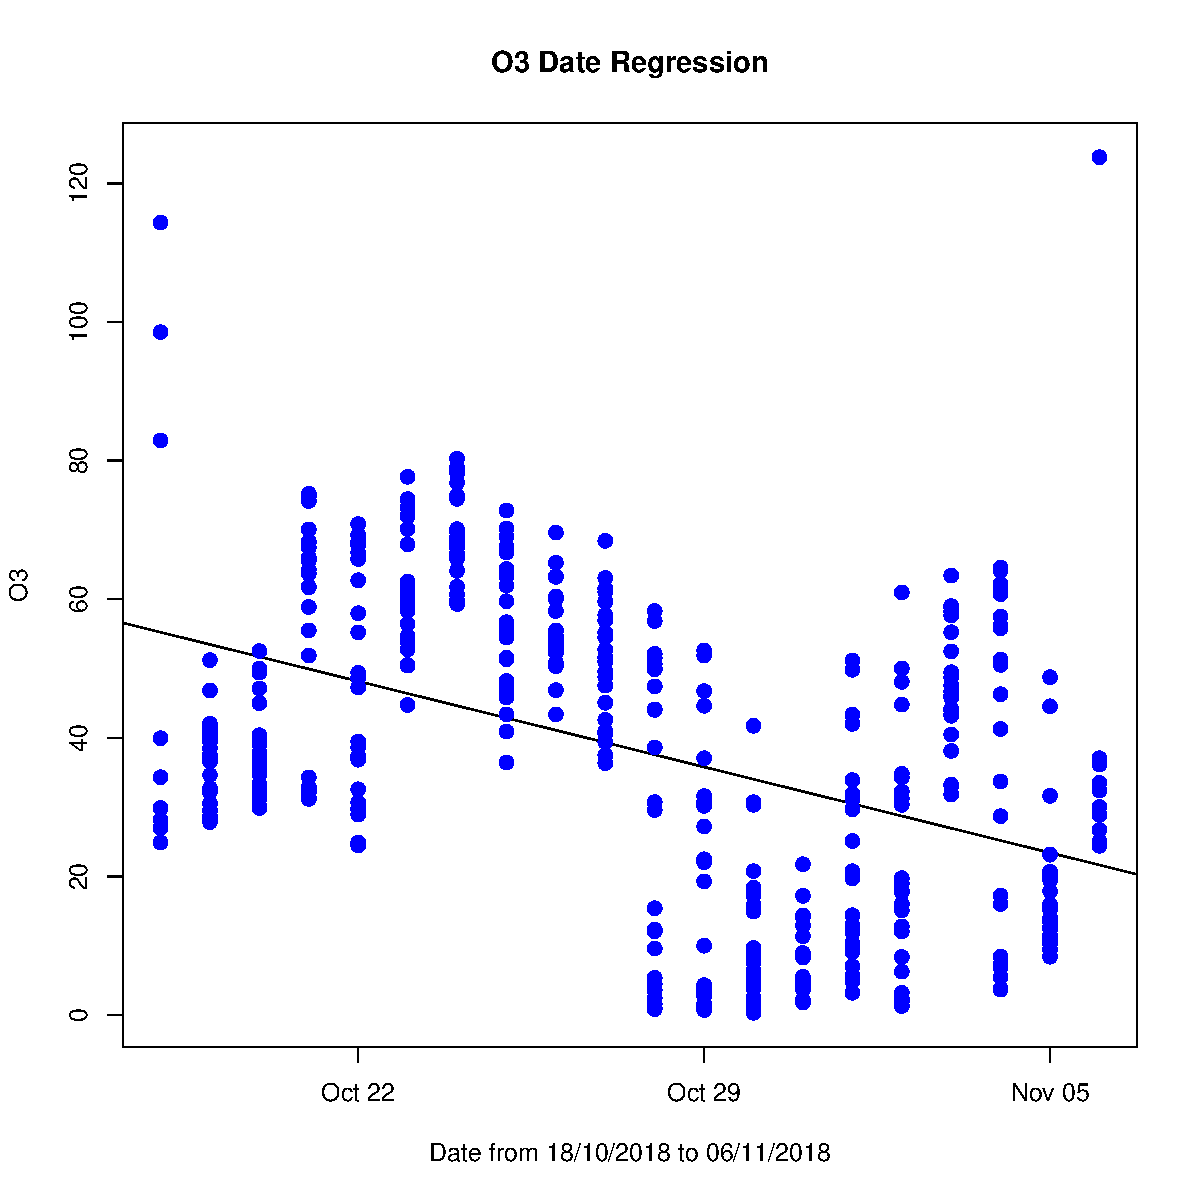
\includegraphics[width=0.4\linewidth]{figures/O3_Date_Regression.pdf}
    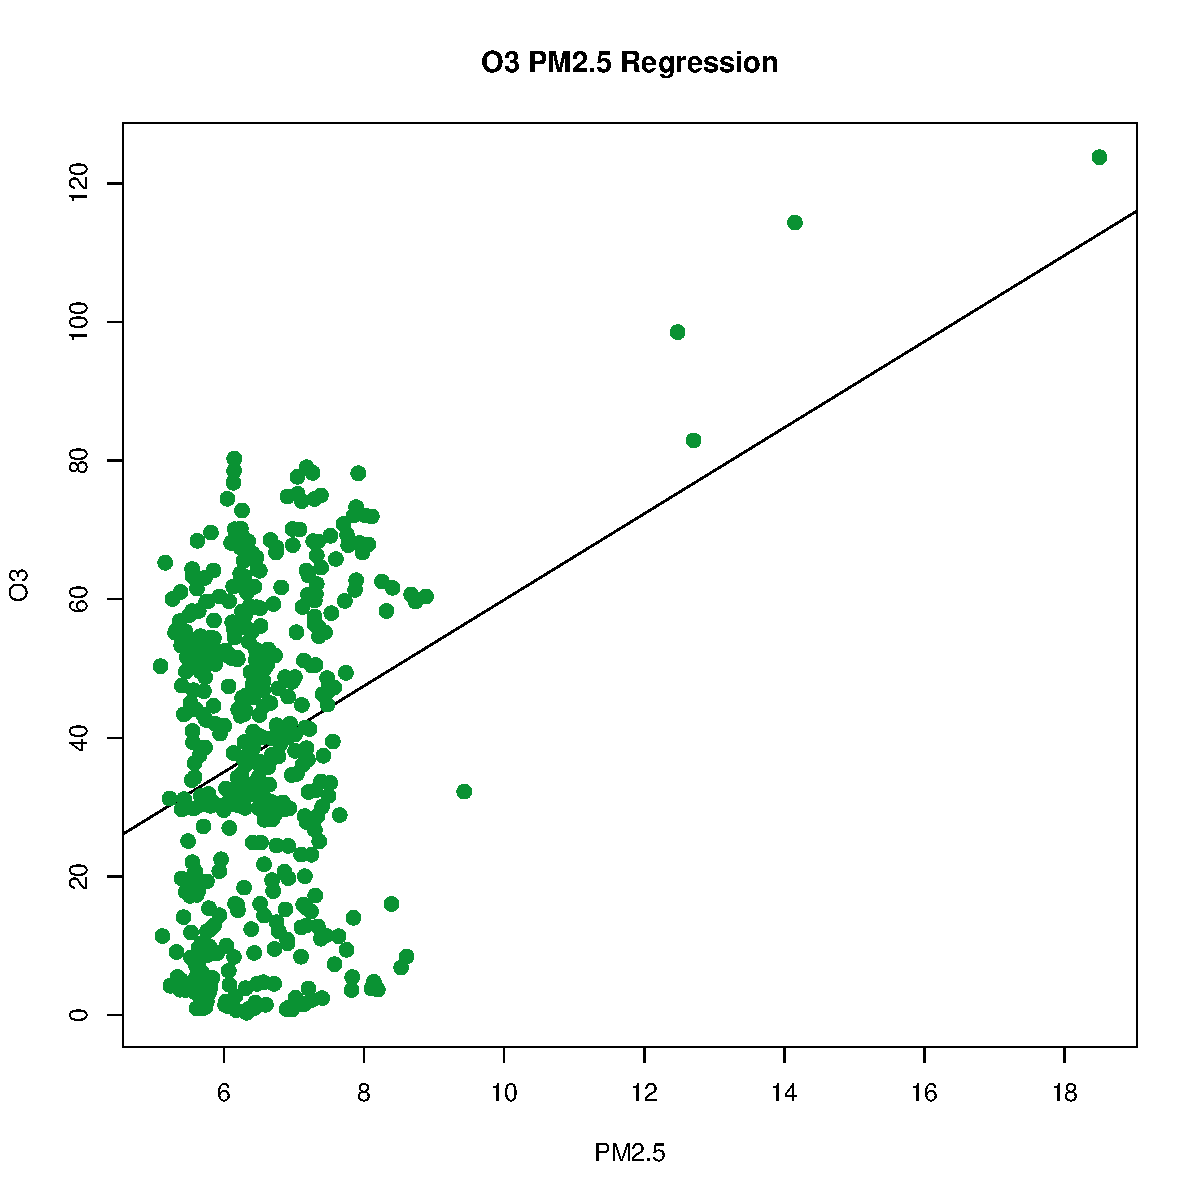
\includegraphics[width=0.4\linewidth]{figures/O3_PM25_Regression.pdf}
    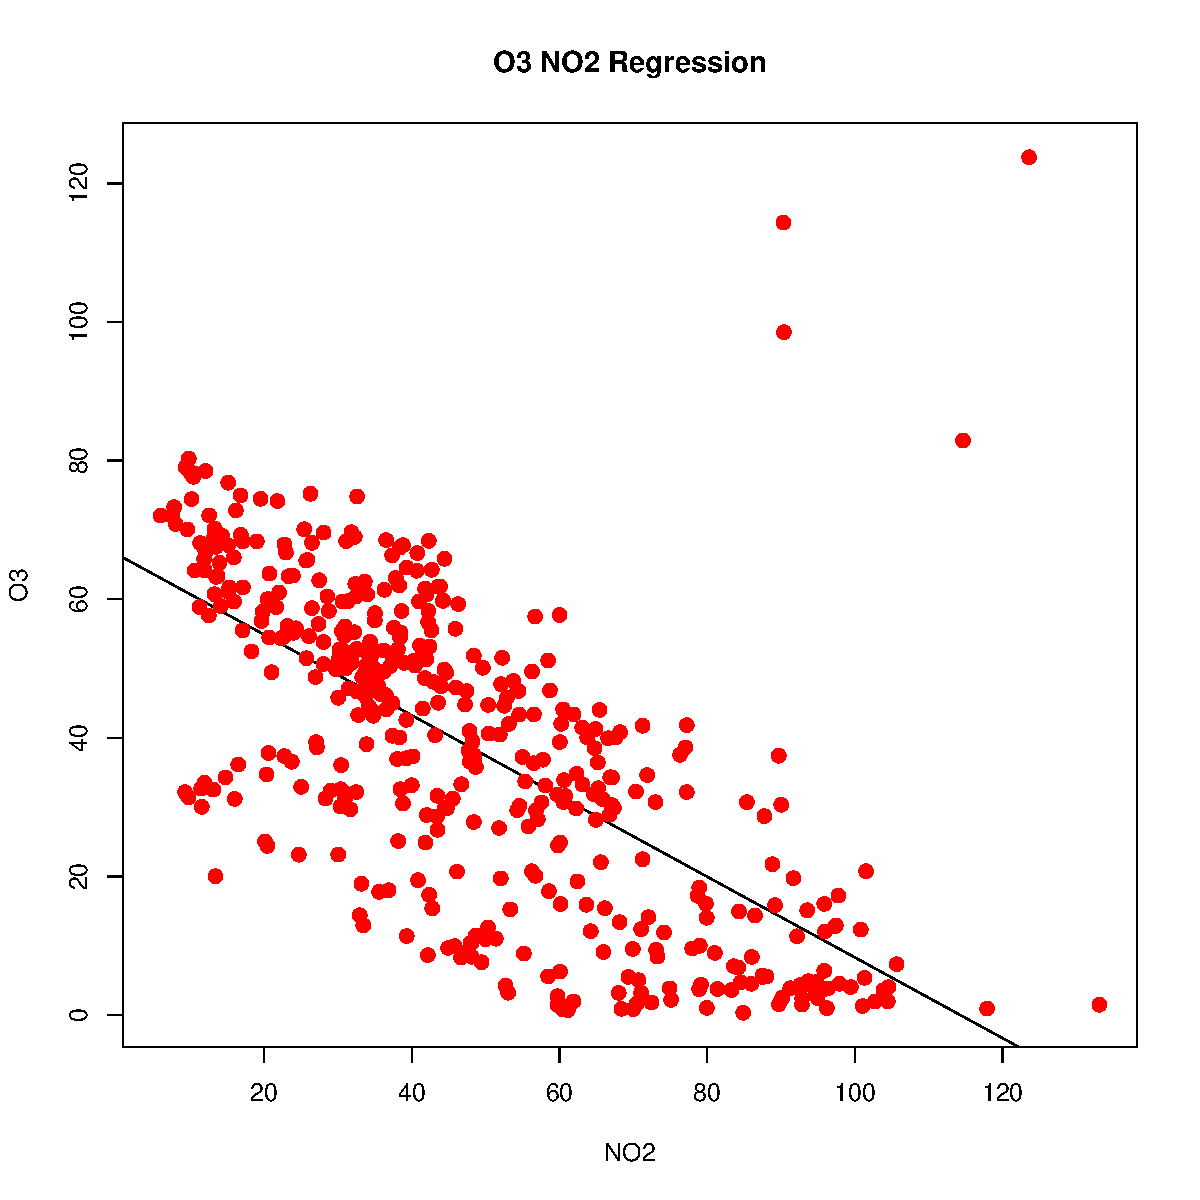
\includegraphics[width=0.4\linewidth]{figures/O3_NO2_Regression.pdf}
    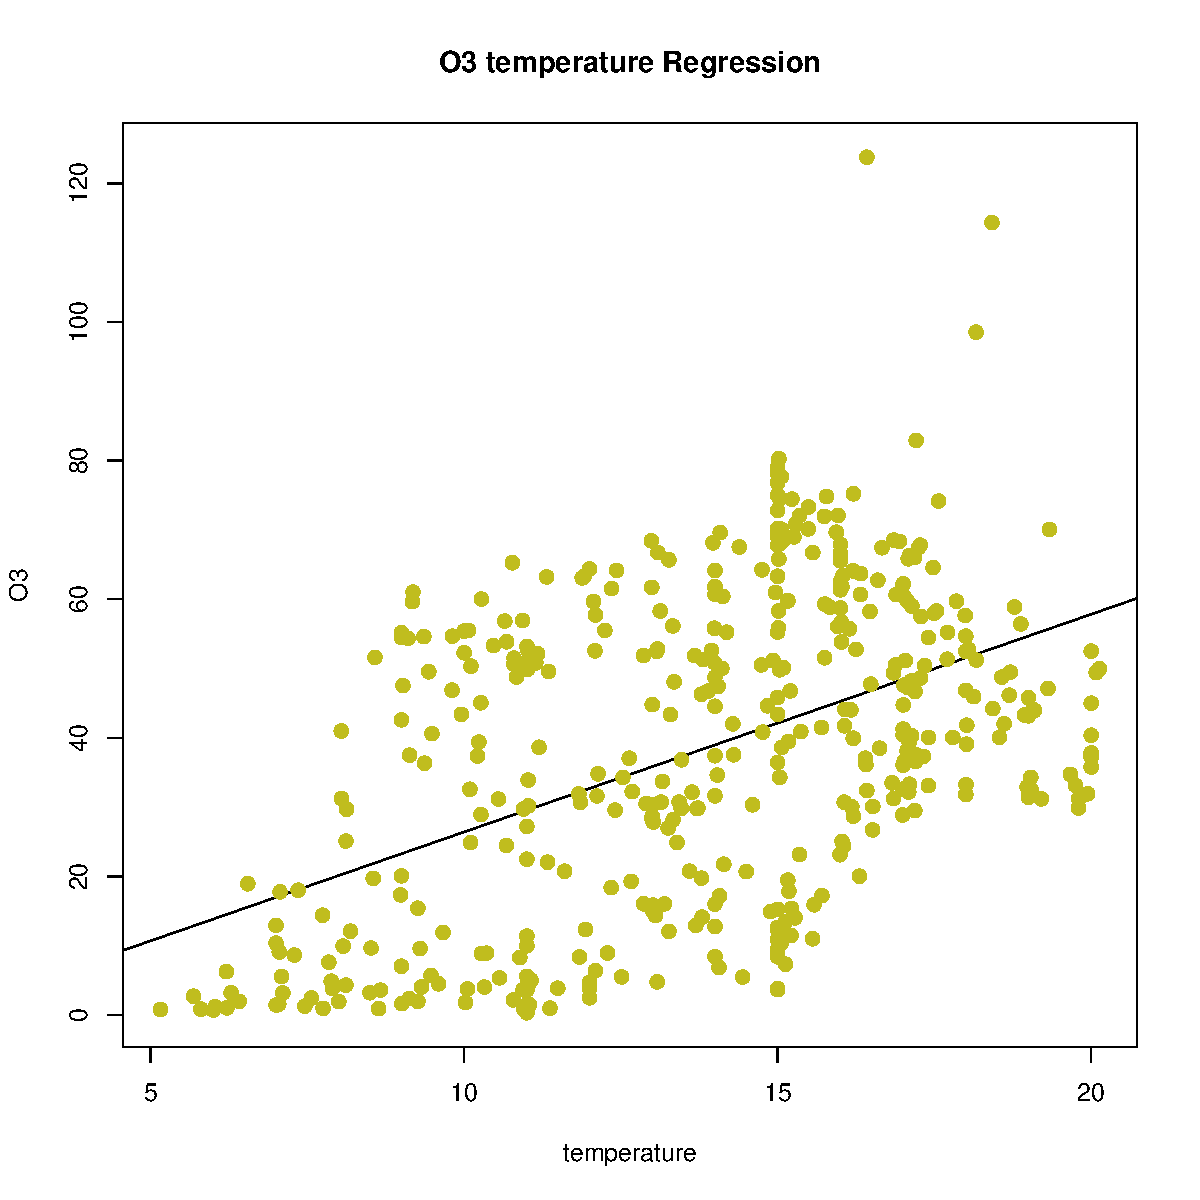
\includegraphics[width=0.4\linewidth]{figures/O3_temperature_Regression.pdf}
    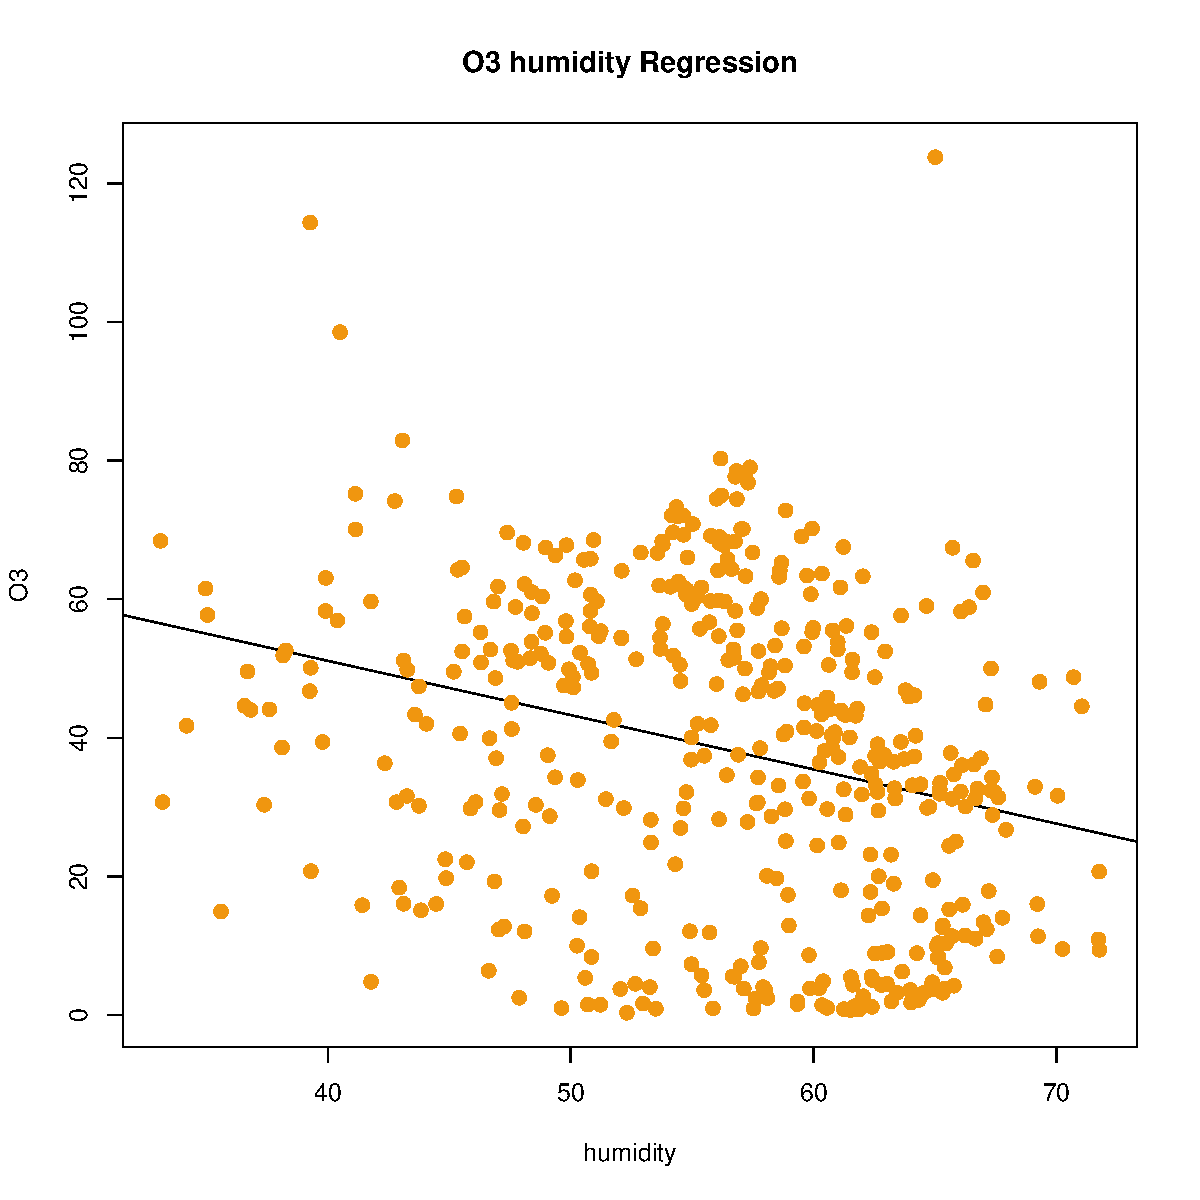
\includegraphics[width=0.4\linewidth]{figures/O3_humidity_Regression.pdf}
    % \caption{}
\end{figure}
% --------------------------------------------------------
% Section 4: multi variable regression forecasting models, visualisation of results
% --------------------------------------------------------
\section{multi variable regression forecasting models, visualisation of results}
\label{sec:multi variable regression forecasting models, visualisation of results}
\begin{figure}[H]
    \centering
    \vspace{-0.35cm}
    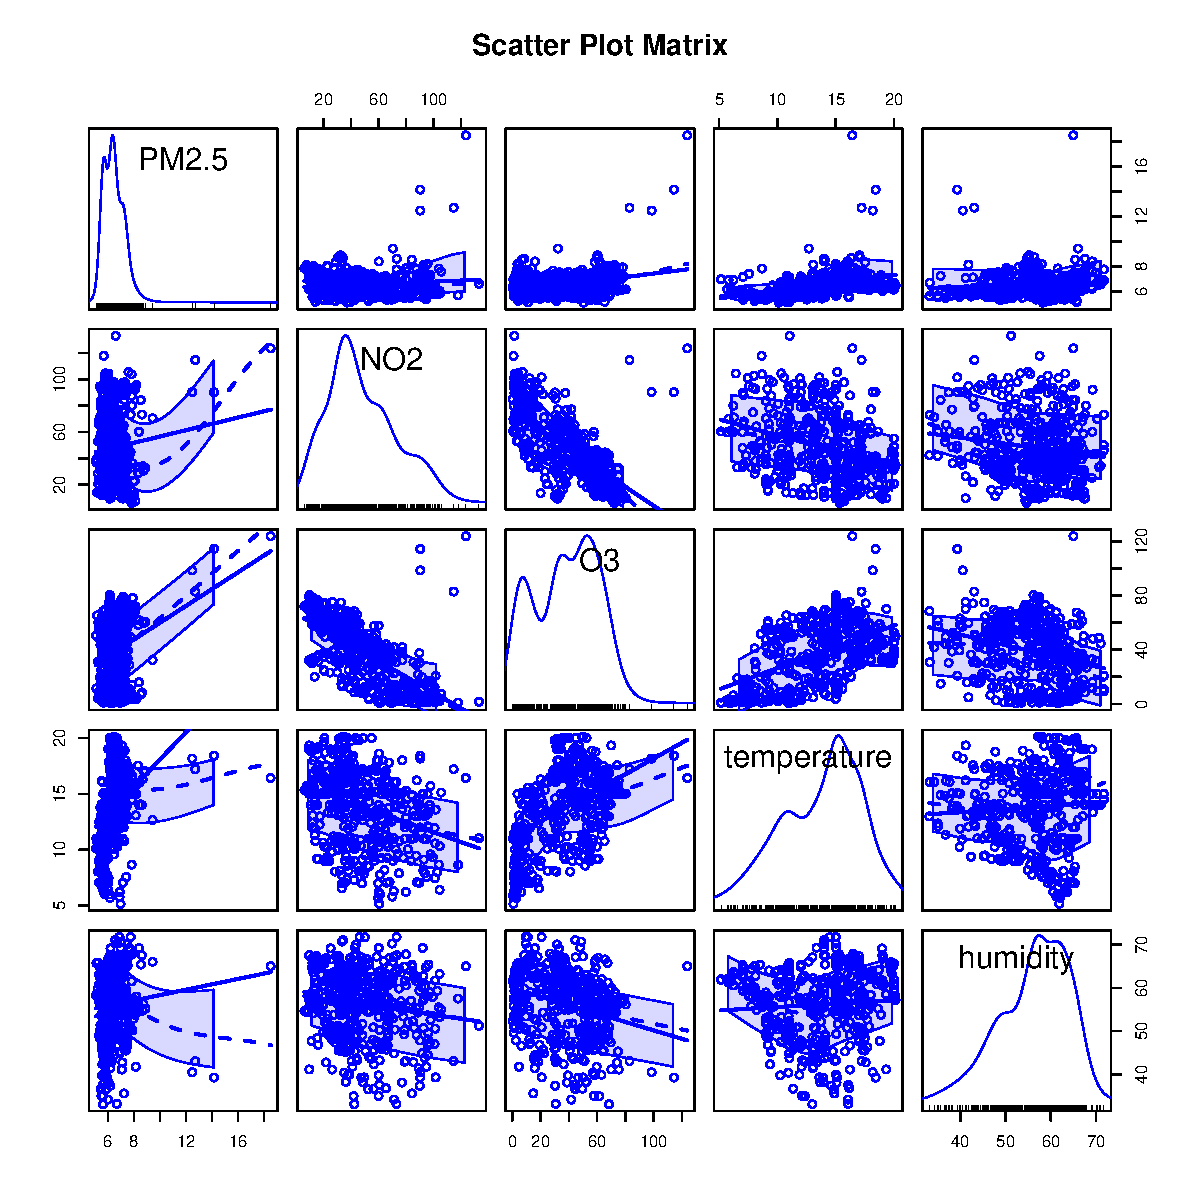
\includegraphics[width=0.4\linewidth]{figures/mul_reg_scatterplotMatrix.pdf}
    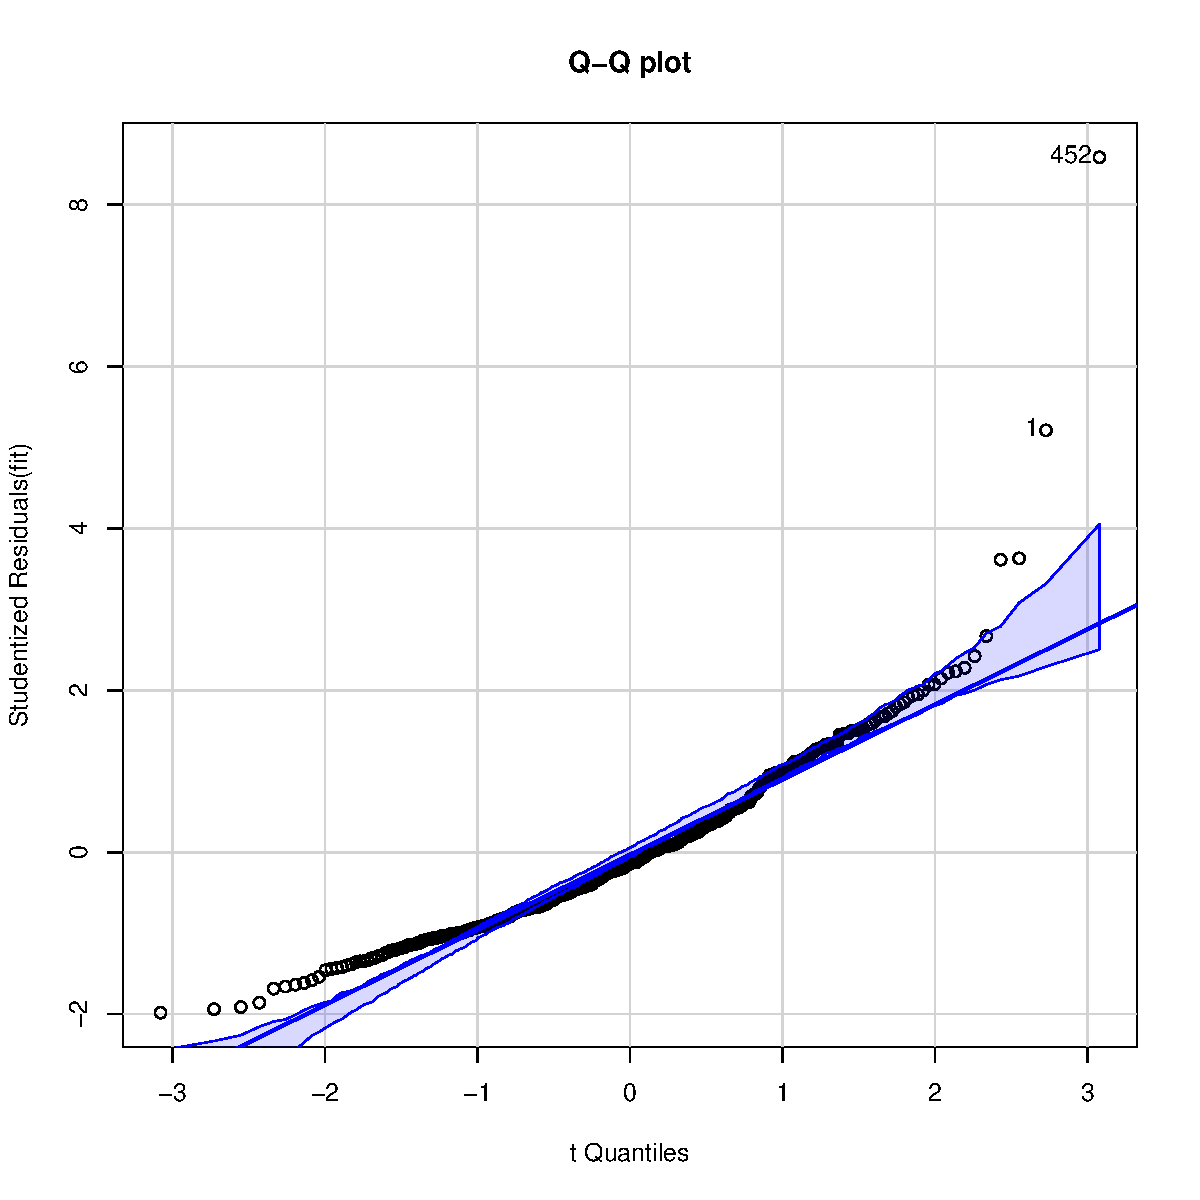
\includegraphics[width=0.4\linewidth]{figures/mul_reg_qqPlot.pdf}
    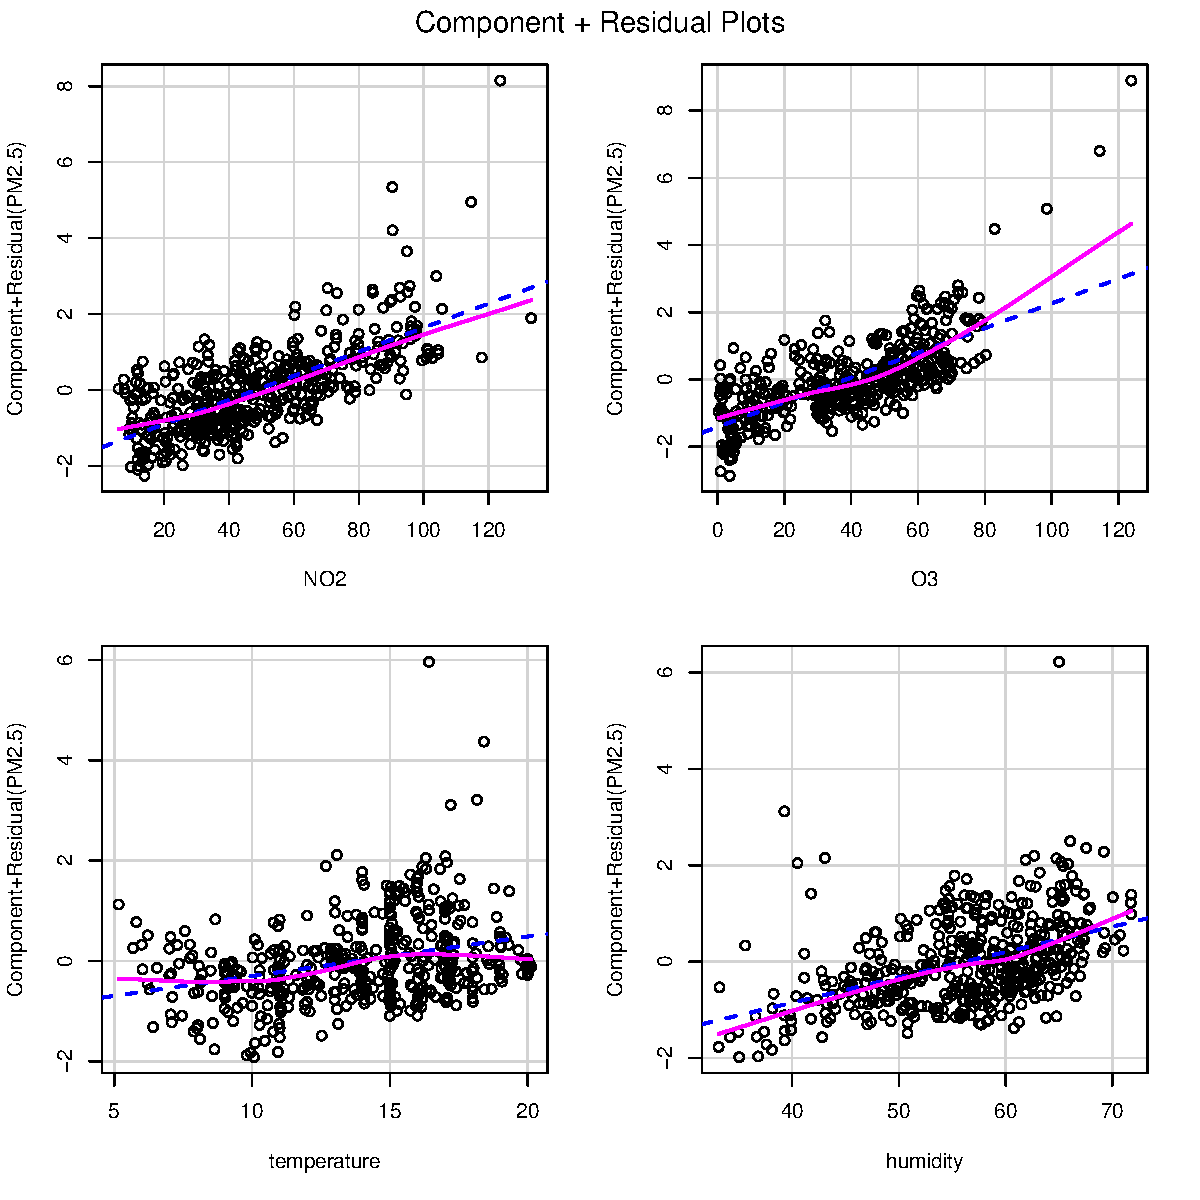
\includegraphics[width=0.4\linewidth]{figures/mul_reg_crPlots.pdf}
    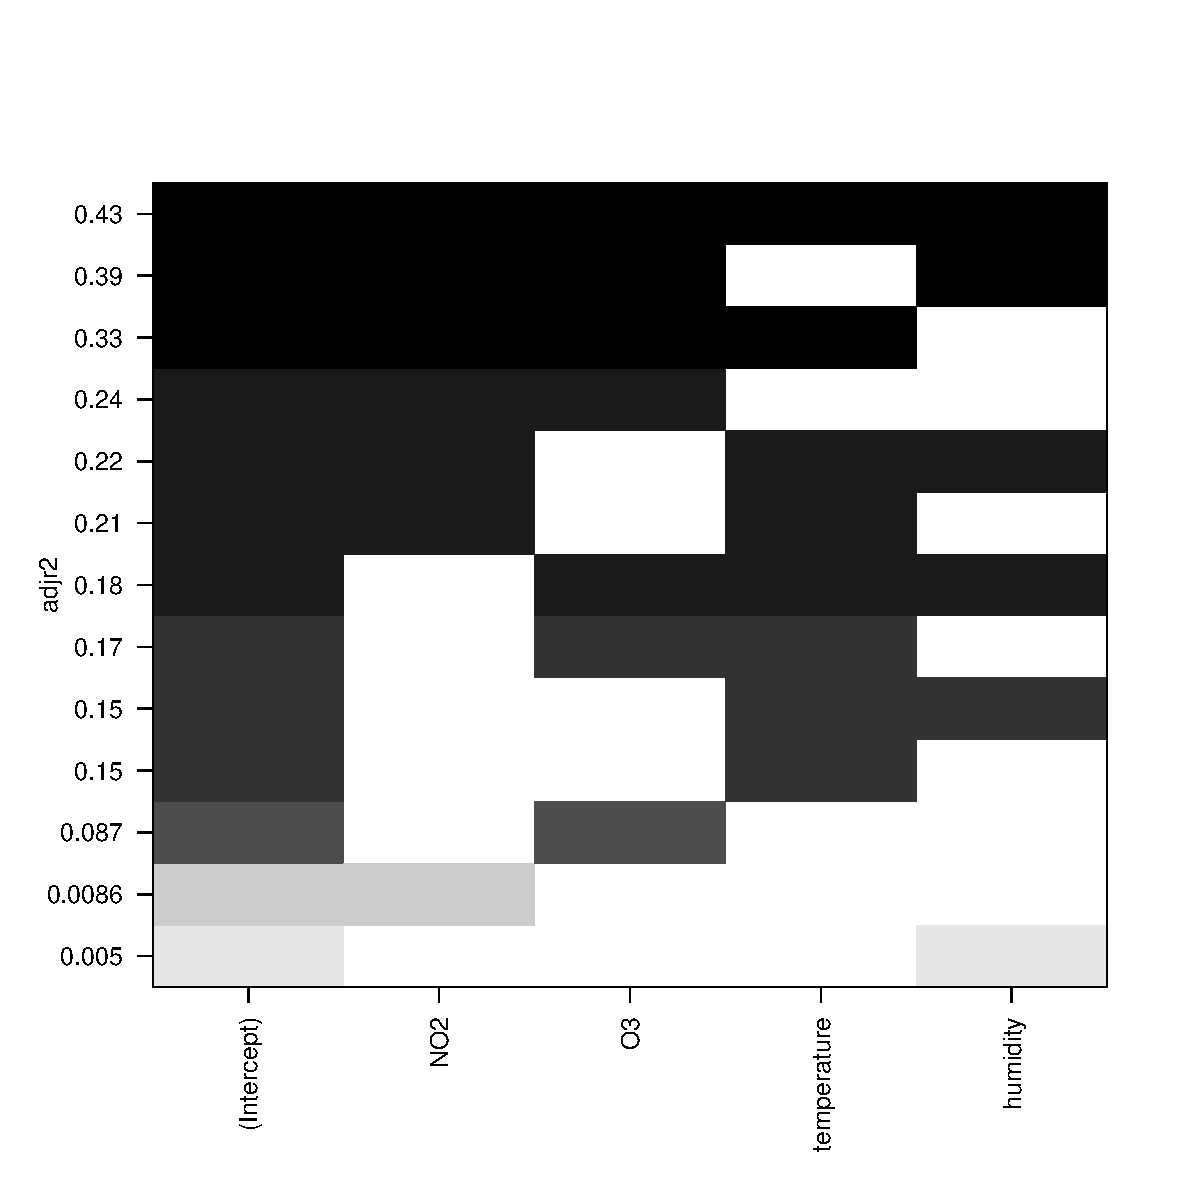
\includegraphics[width=0.4\linewidth]{figures/mul_reg_adjr2.pdf}
    % \caption{}
\end{figure}



% --------------------------------------------------------
% Section 5: model performance and discussion of results
% --------------------------------------------------------
\section{model performance and discussion of results}
\label{sec:model performance and discussion of results}


% --------------------------------------------------------
% Section 6: Conclusions
% --------------------------------------------------------
\section{Conclusions}
    
\newpage
\bibliographystyle{IEEEtran}
\bibliography{References}

\end{document}